%!TEX root=./pfc.tex
\chapter[Diseño del sistema]{\label{}
Diseño del sistema}

\section{Diseño de la base de datos}

\subsection{Modelo Conceptual}

Se trata de representar la información de las distintas Wikicodes que puede almacenar un sistema e-learning, para que el sistema pueda acceder a la información referente al código fuente que están modificando los usuarios, así como para posibilitar una mejor consulta de estadísticas, histórico. También nos servirá para almacenar la información respecto a la compilación del código.

\subsubsection{Análisis de los tipos de entidad}

En principio, del análisis de requisitos del capítulo anterior pueden ser extraídos los siguientes tipos de entidad, como se muestra en la figura 4.1:

\begin{description}
	\item{\textbf{Tipo de entidad}} \emph{wikicode}: el cual representa el módulo que se ha creado durante este proyecto y que se puede definir como \emph{``el entorno de programación colaborativo''}. Se van a considerar como atributos de esta entidad un identificador secuencial que nos proporcione una clave para poder hacer referencia a él. También necesitaremos la información que se corresponde al curso en el que ha querido ser creado. 
	
	Posteriormente necesitaremos una serie de atributos informativos como es la hora de creación, de modificación, nombre, lenguaje de la Wikicode y tipo de Wikicode. 

\begin{figure}[h]
	\centering
	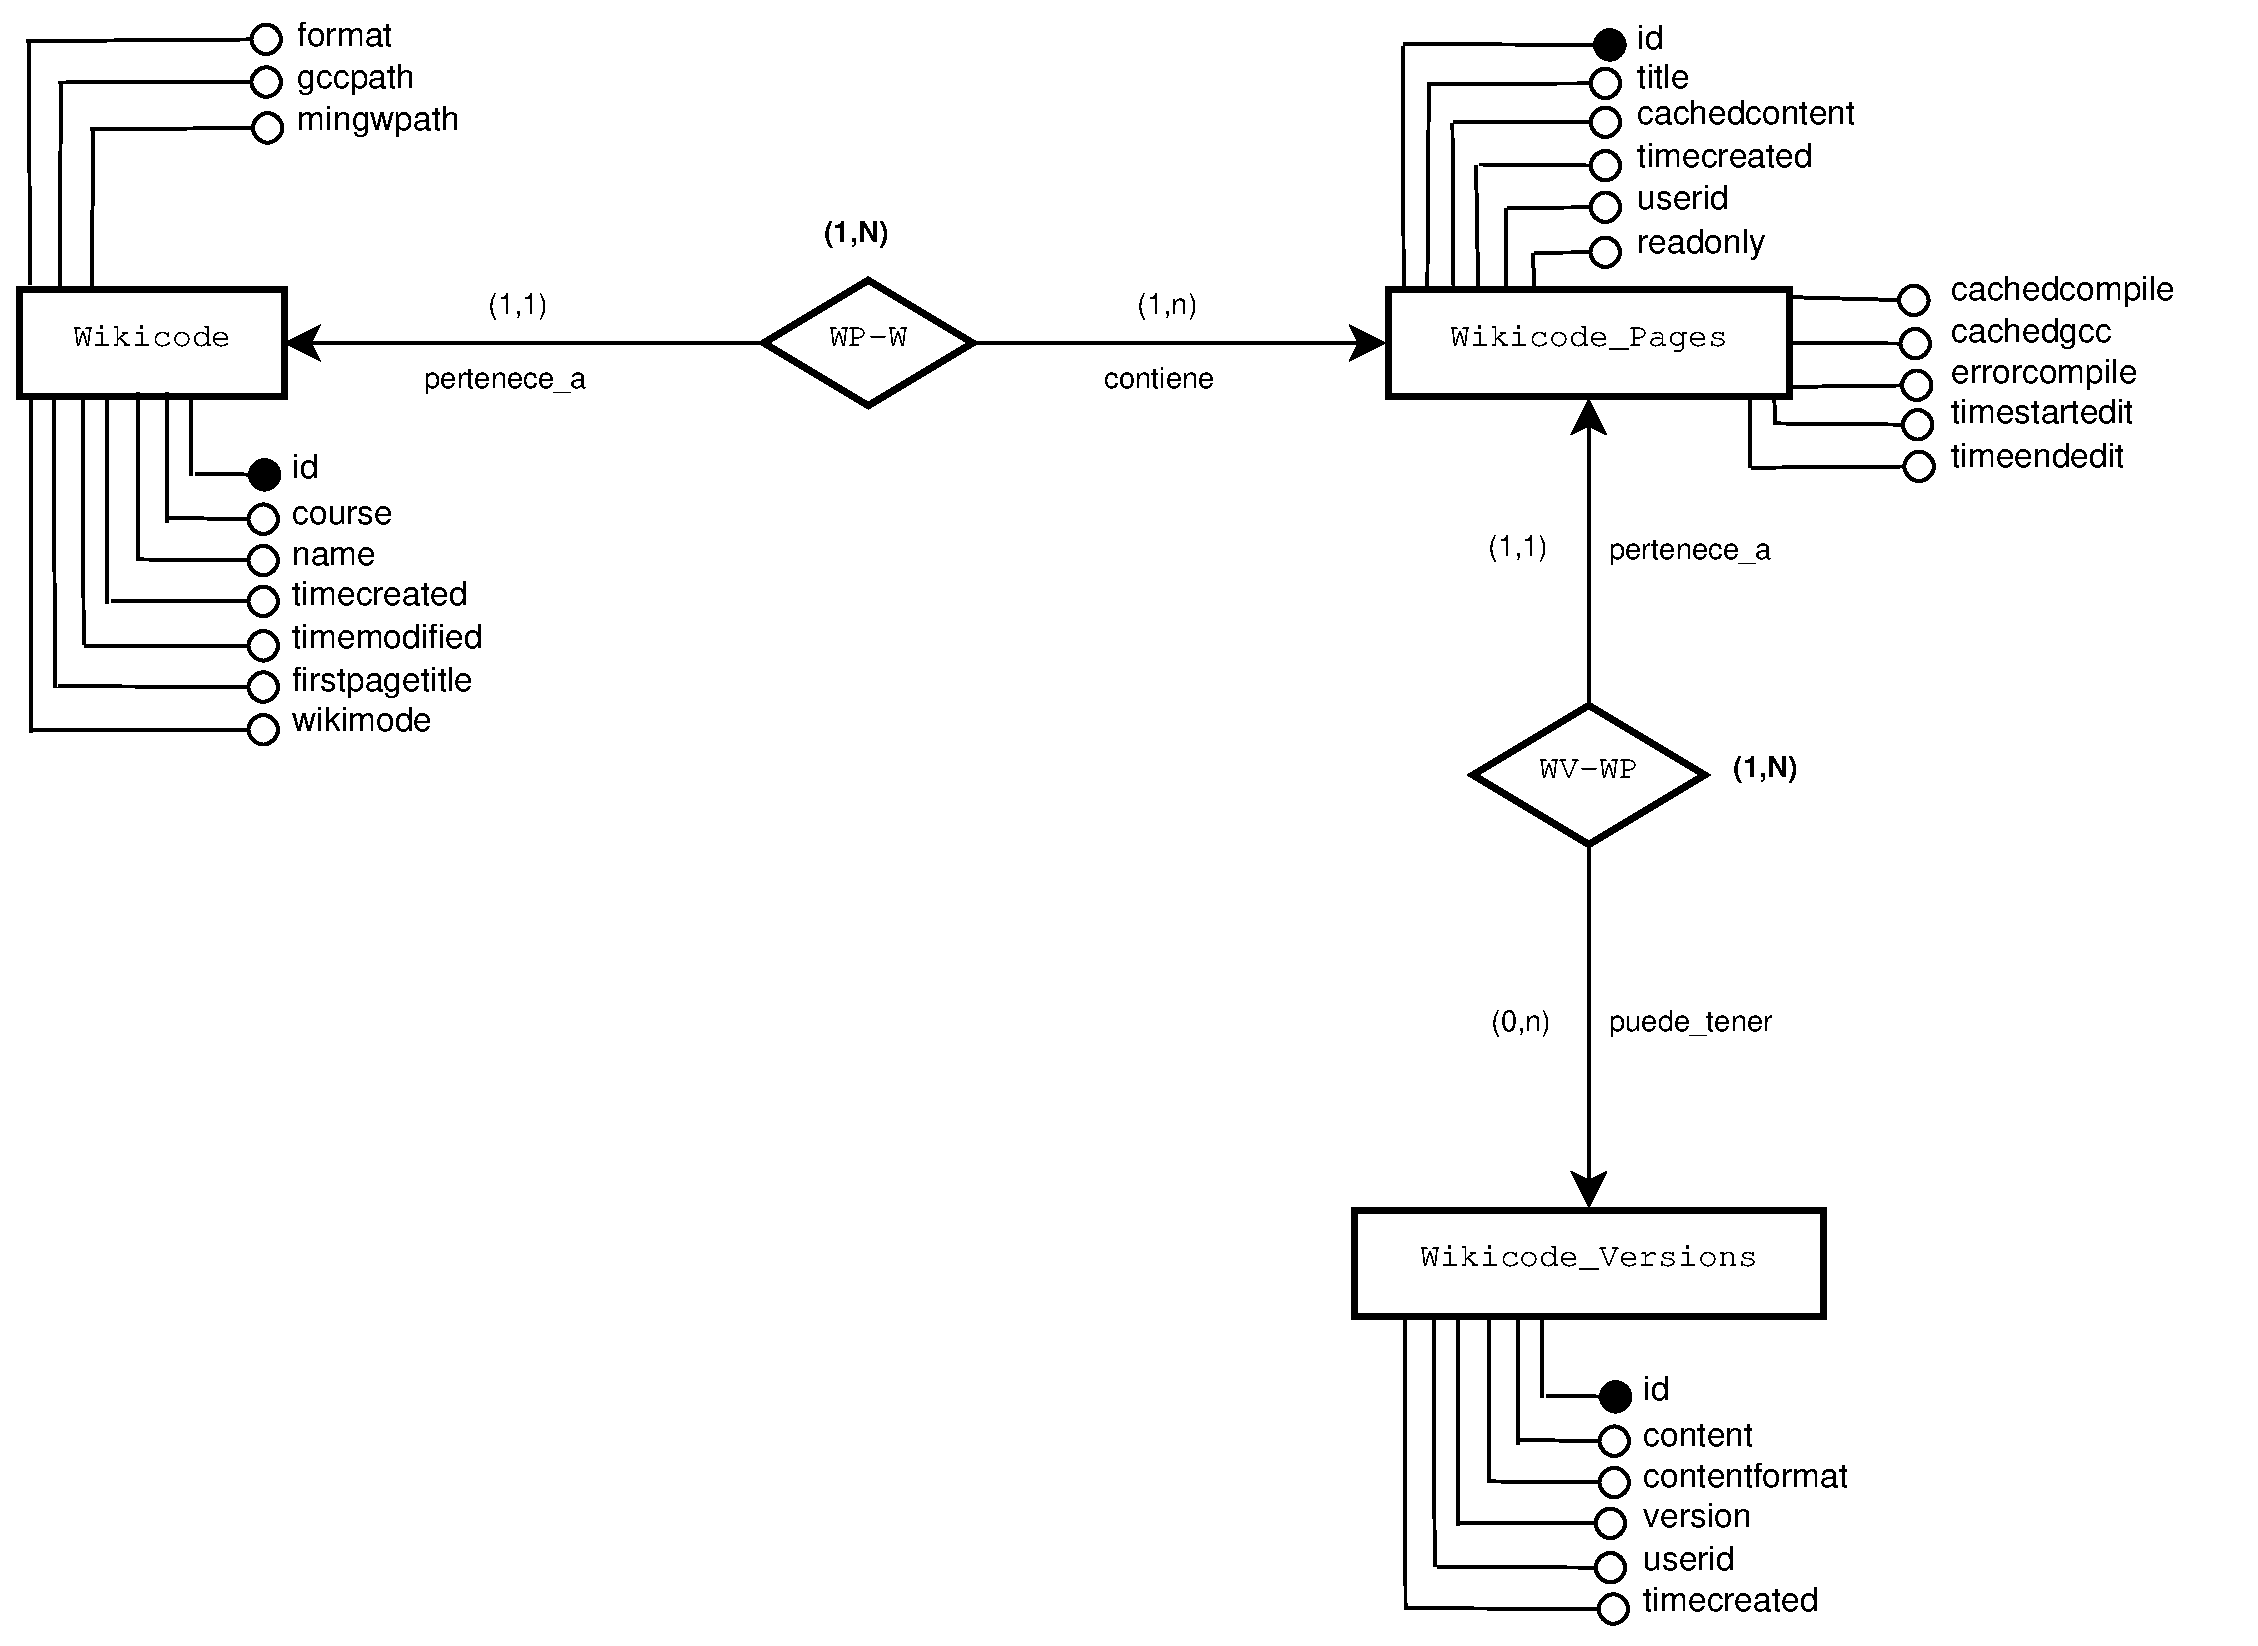
\includegraphics[width=\textwidth]{./img/EER.eps}
	\caption{Esquema EE-R del modelo conceptual del módulo Wikicode}
\end{figure}
	
	También contará con los atributos correspondiente a la parametrización del compilador, donde dividiremos en el que se querrá usar para Windows y el que se querrá usar para entornos Unix.
	
	\item{\textbf{Tipo de entidad}} \emph{wikicode\_pages}: el cual representa al objeto del mundo real \emph{página} que representa \emph{``el código fuente editado de modo colaborativo en lenguaje C''}. Se van a considerar como atributos el título que se haya considerado al crearse así como el contenido del código. También será necesario una serie de información estadística y de información como es saber el identificador del usuario que lo ha creado, el número de visualizaciones que ha tenido ese código y si sólo queremos que sea de lectura.
	
	También es importante contar con la información del compilador, por lo que se almacenará el código que se ha enviado al compilador y la salida que ha producido este al enviarle dicho código como parámetro. Por último también contaremos con la información estadística necesaria para la visualización de los logs: Hora de primera edición, Hora de última edición y Número de errores de compilación.
	
	\item{\textbf{Tipo de entidad}} \emph{wikicode\_versions}: el cual representa el objeto del mundo real \emph{version} que representa \emph{``el código fuente colaborativo en lenguaje C en un momento específico del tiempo''}. Esta información es necesaria para mantener un histórico por lo que únicamente contaremos como atributos el código fuente de dicha versión, el tipo de contenido, el número de versión que se trata, la hora en que fue creada dicha versión y la información referente al usuario que creó esta entrada.
\end{description}

\subsubsection{Análisis de los tipos de interrelación}

Los tipos de entidad antes mencionados se encuentran relacionados de la siguiente forma:

\begin{description}
	\item{\textbf{Tipo de interrelación}} \emph{Wikicode/Wikicode\_Pages} \textbf{W-WP}: el cual relaciona los tipos de entidad \emph{Wikicode} y \emph{Wikicode\_Pages}, la interrelación es del tipo \emph{1:N}, ya que una página pertenece a una única wikicode, por tanto, el tipo de entidad \emph{Wikicode\_Pages} participa con las cardinalidades \emph{(1,1)} en este tipo de interrelación, mientras que en una Wikicode pueden existir muchas páginas debido a la creación de grupos. Se considera que una Wikicode no tiene sentido sin que existan páginas en su interior, por lo que el tipo de entidad \emph{Wikicode} participara en el tipo de interrelación \emph{W-WP} con las cardinalidades \emph{(1,n)} como se puede observar en la figura 4.1.
	
	\item{\textbf{Tipo de interrelación}} \emph{Wikicode\_Pages/Wikicode\_Version} \textbf{WP-WV}: el cual relaciona los tipos de entidad \emph{Wikicode\_Pages} y \emph{Wikicode\_Versions}, la interrelación es del tipo \emph{1:N}, ya que una versión del histórico pertenece a un único código fuente, por tanto, el tipo de entidad \emph{Wikicode\_Versions} participa con las cardinalidades \emph{(1,1)} en este tipo de interrelación, mientras que de un código fuente pueden existir muchas versiones en un histórico. No hay necesidad de que un código fuente tenga almacenada información en su histórico, por lo que el tipo de entidad \emph{Wikicode\_Pages} participara en el tipo de interrelación \emph{WP-WV} con las cardinalidades \emph{(0,n)} como se puede observar en la figura 4.1.
\end{description}

\newpage

\subsection{Modelo Relacional}

Una vez realizado el modelo conceptual se va a construir el modelo relacional del problema considerado.

\subsubsection{Tabla Wikicode}

La tabla \emph{Wikicode} se forma a partir del tipo de entidad \emph{Wikicode}. Esta tabla incluye los atributos \emph{id, course, name, timecreated, timemodified, firstpagetitle, wikimode, format, gccpath} y \emph{mingwpath} que son tomados del tipo de entidad antes mencionado (regla RTECAR-1).

La clave principal de la tabla es el atributo \emph{id}, no considerándose, en este caso, ningún otro atributo que pueda ser utilizado como identificador alternativo, y ninguno de los atributos de esta tabla mantiene referencia alguna con los atributos de las otras tablas. La tabla \emph{Wikicode} queda de la siguiente forma:

\begin{description}
	\item{\textbf{Wikicode}} \emph{(\underline{id}, course, name, timecreated, timemodified, firstpagetitle, wikimode, format, gccpath, mingwpath)}
\end{description}

\subsubsection{Tabla Wikicode\_Pages}

La tabla \emph{Wikicode\_Pages} se forma a partir del tipo de entidad del mismo nombre tomando los atributos de este tipo de entidad (regla RTECAR-1), además de:

\begin{itemize}
	\item El atributo identificador de la tabla \emph{Wikicode} con la cual mantiene una relación uno a muchos (regla RTECAR-3.1).
\end{itemize}

La clave principal de la tabla es el atributo \emph{id}, no considerándose, en este caso, ningún otro atributo que pueda ser utilizado como identificador alternativo.

\begin{description}
	\item{\textbf{Wikicode\_Pages}} \emph{(\underline{id}, title, cachedcontent, timecreated, userid, readonly, cachedcompile, cachedgcc, errorcompile, timestartedit, timeendedit, \textbf{subwikiid})}
\end{description}

\subsubsection{Tabla Wikicode\_Versions}

La tabla \emph{Wikicode\_Versions} se forma a partir del tipo de entidad del mismo nombre tomando los atributos de este tipo de entidad (regla RTECAR-1), además de:

\begin{itemize}
	\item El atributo identificador de la tabla \emph{Wikicode\_Pages} con la cual mantiene una relación uno a muchos (regla RTECAR-3.1).
\end{itemize}

La clave principal de la tabla es el atributo \emph{id}, no considerándose, en este caso, ningún otro atributo que pueda ser utilizado como identificador alternativo.

\begin{description}
	\item{\textbf{Wikicode\_Pages}} \emph{(\underline{id}, content, contentformat, version, timecreated, \textbf{pageid})}
\end{description}

\subsection{Normalización del modelo}

\begin{description}
	\item{\textbf{Table} \emph{Wikicode}}: esta tabla se encuentra en FNBC, pues todos los atributos son atómicos (FN1) y las dependencias funcionales son completas.
\end{description}

\begin{description}
	\item{\textbf{Table} \emph{Wikicode\_Pages}}: al igual que en el caso anterior, esta tabla se encuentra en FNBC.
\end{description}

\begin{description}
	\item{\textbf{Table} \emph{Wikicode\_Versions}}: por el mismo razonamiento esta tabla se encuentra en FNBC.
\end{description}

\begin{figure}[h]
	\centering
	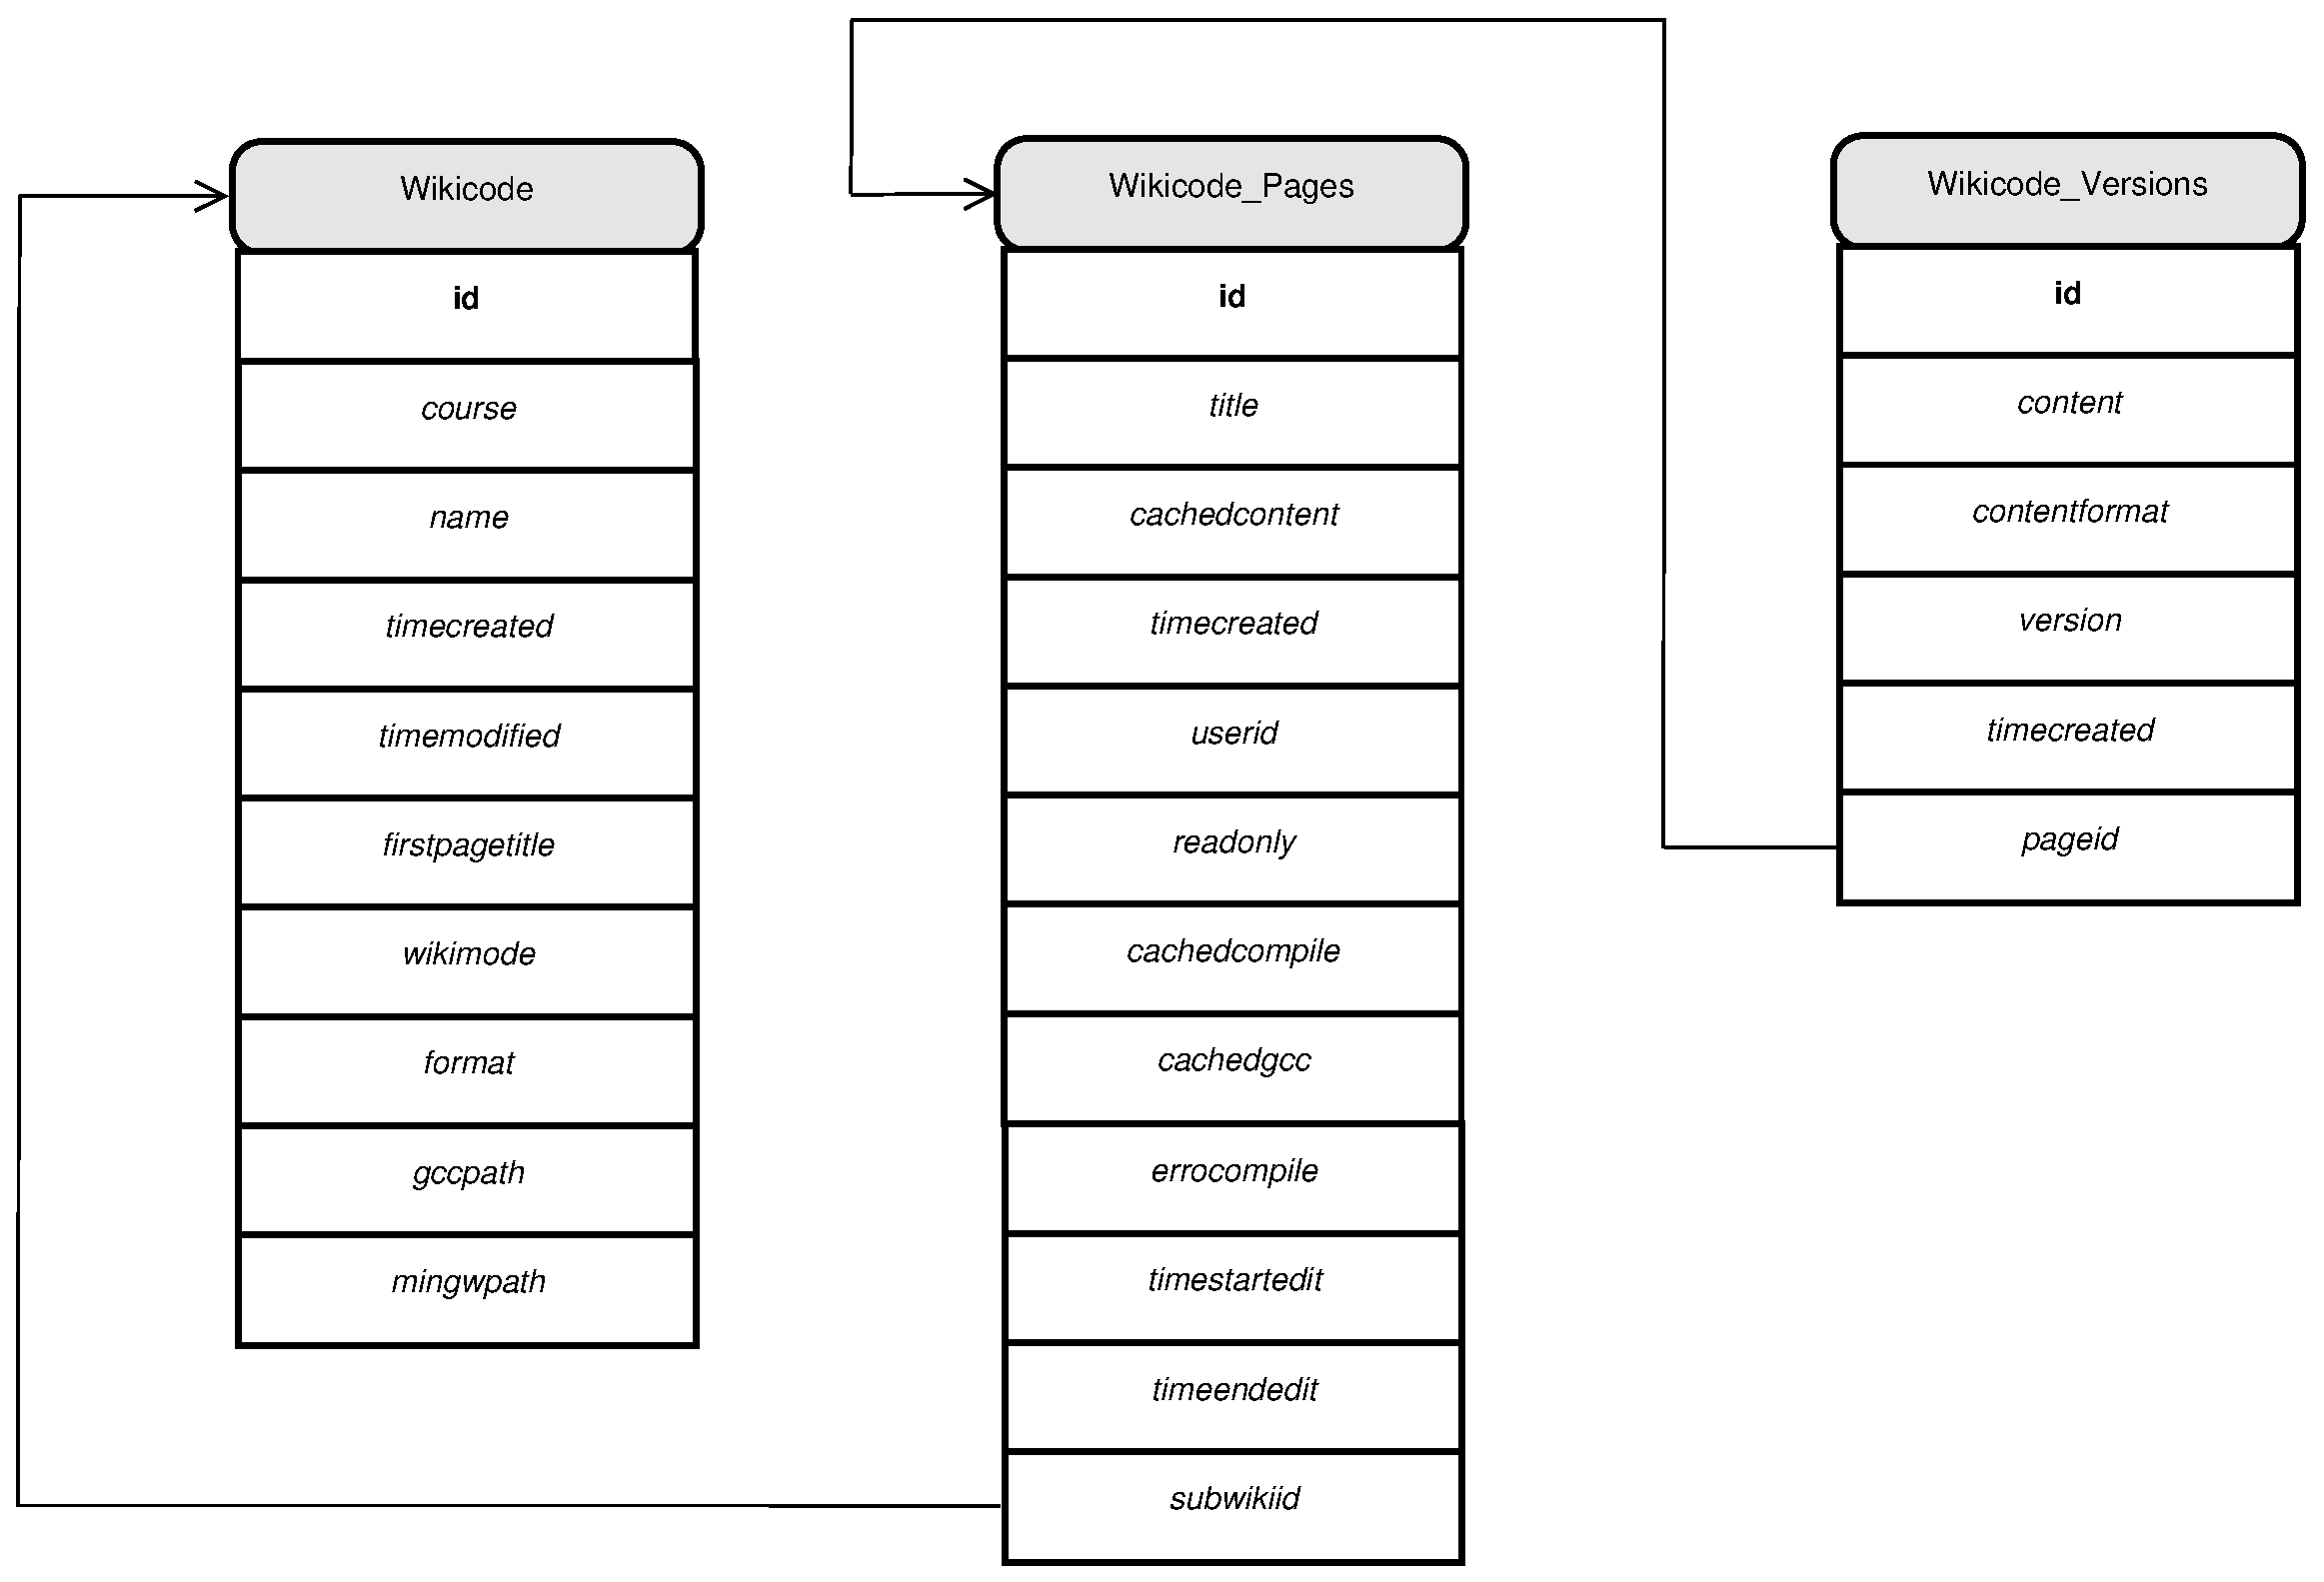
\includegraphics[width=\textwidth]{./img/ERelacional.eps}
	\caption{Diagrama relacional para el módulo Wikicode}
\end{figure}

\section{Descripción del resultado final del interfaz}

En este apartado se describirá cómo interactúa el sistema con el usuario, definiendo la estructura y comportamiento del interfaz. Aunque el diseño de esta interfaz no es uno de los objetivos primordiales del proyecto, se ha intentado realizar un diseño de manera que se facilite el manejo del sistema al usuario aprovechando las características del entorno Moodle. Además, para la parte en que el usuario va a editar el código fuente, se ha simulado un editor con características similares a cualquier otro editor de código que se pueda encontrar.

\subsection{Descripción del interfaz}

En cuanto a la estructura general del interfaz del módulo desarrollado, hay que tener en cuenta que nuestro proyecto se ha centrado en la realización de un módulo que pueda ser utilizado en Moodle.

De esta manera, el diseño de los módulos por defecto de Moodle se ha tomado como base para el desarrollo del nuevo bloque. Este hecho permite conseguir homogeneidad del sistema de manera que todos los bloques y elementos se encuentren en consonancia.

Por tanto, nos limitaremos a hablar del diseño realizado para el bloque en cuestión sin especificar características especiales de Moodle.

\newpage
\subsection{Descripción de las pantallas del interfaz}

\subsubsection{Pantalla principal}

Al tratarse de un módulo la creación de una Wikicode y su posterior selección será igual a la otro cualquiera (Foro, Wiki, Chat, Cuestionario, etc.). En la siguiente figura se muestra como se añadiría una nueva Wikicode a un curso ya creado:

\begin{figure}[h]
	\centering
	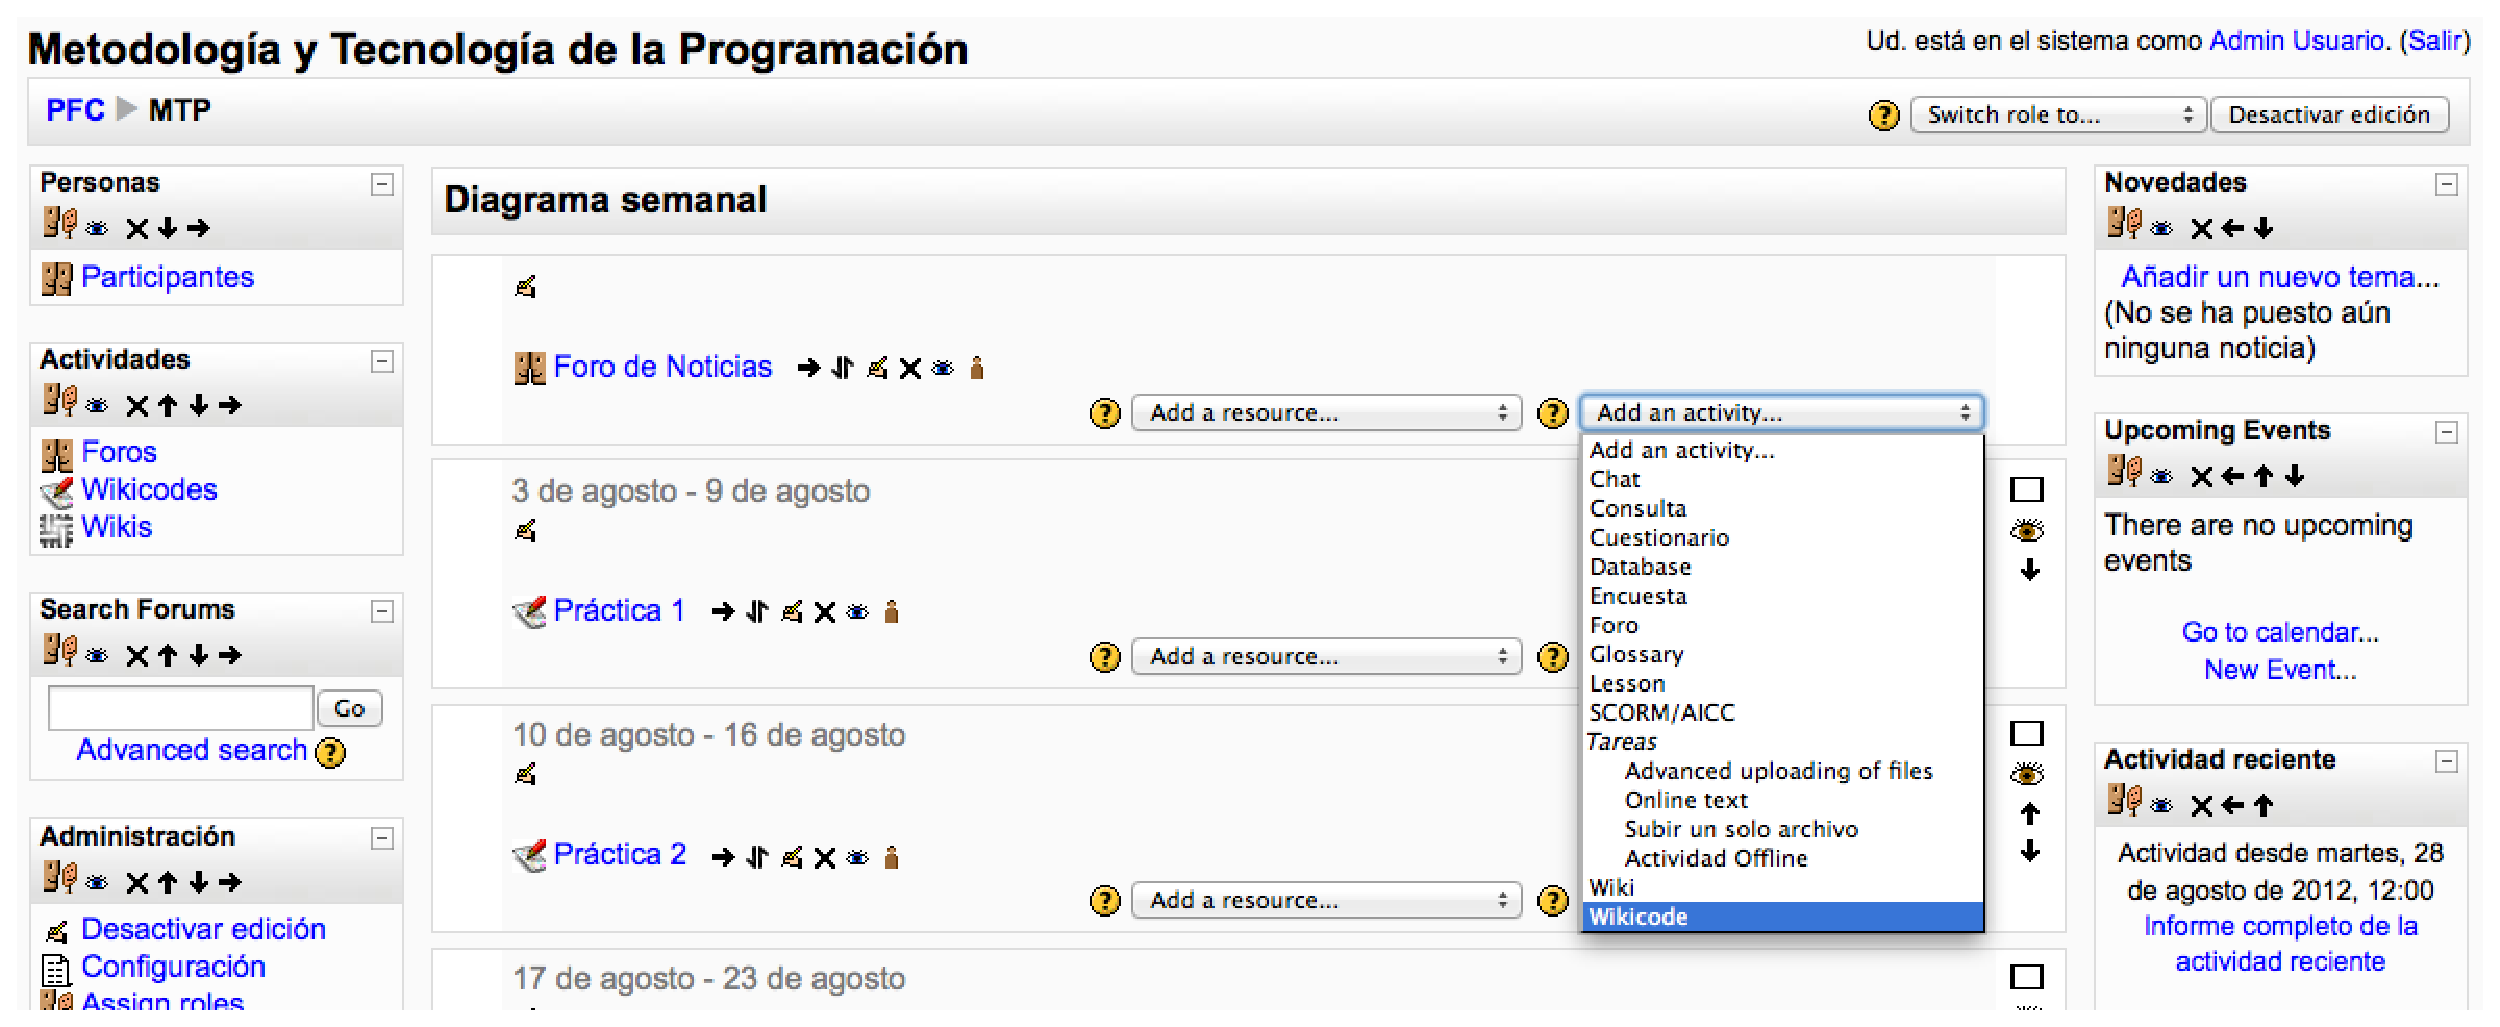
\includegraphics[width=\textwidth]{./img/c4main.eps}
	\caption{Pantalla principal de un curso Moodle añadiendo una Wikicode}
\end{figure}

\subsubsection{Pantalla configuración y parametrización}

Cuando se accede a la opción de crear una nueva Wikicode se accede a la pantalla de configuración del módulo. Este formulario contendrá todas las variables para la creación del entorno colaborativo deseado. En concreto las variables a tener en cuenta será la elección del nombre y la descripción del mismo, la posibilidad de agrupamiento con respecto a una Wikicode (eligiendo de una lista) y la parametrización del compilador que desea usarse.

Para ayudar al tutor, se ha optado por una ayuda automática a la hora de parametrizar los compiladores, tomando siempre por defecto el valor que haya sido usado un mayor número de veces con anterioridad. Si nunca se ha usado ninguno por defecto aparecerá el nombre del compilador recomendado.

\newpage

En la siguiente figura se muestra la pantalla de configuración que se presenta cuando se decide crear una nueva Wikicode:

\begin{figure}[h]
	\centering
	\includegraphics[width=0.68\textwidth]{./img/c4param.eps}
	\caption{Pantalla de configuración y parametrización Wikicode}
\end{figure}

Además, a partir de la versión 2 de Moodle se ha actualizado el módulo para que cada opción traiga consigo una ayuda que nos explique la funcionalidad de cada variable.

\begin{figure}[h]
	\centering
	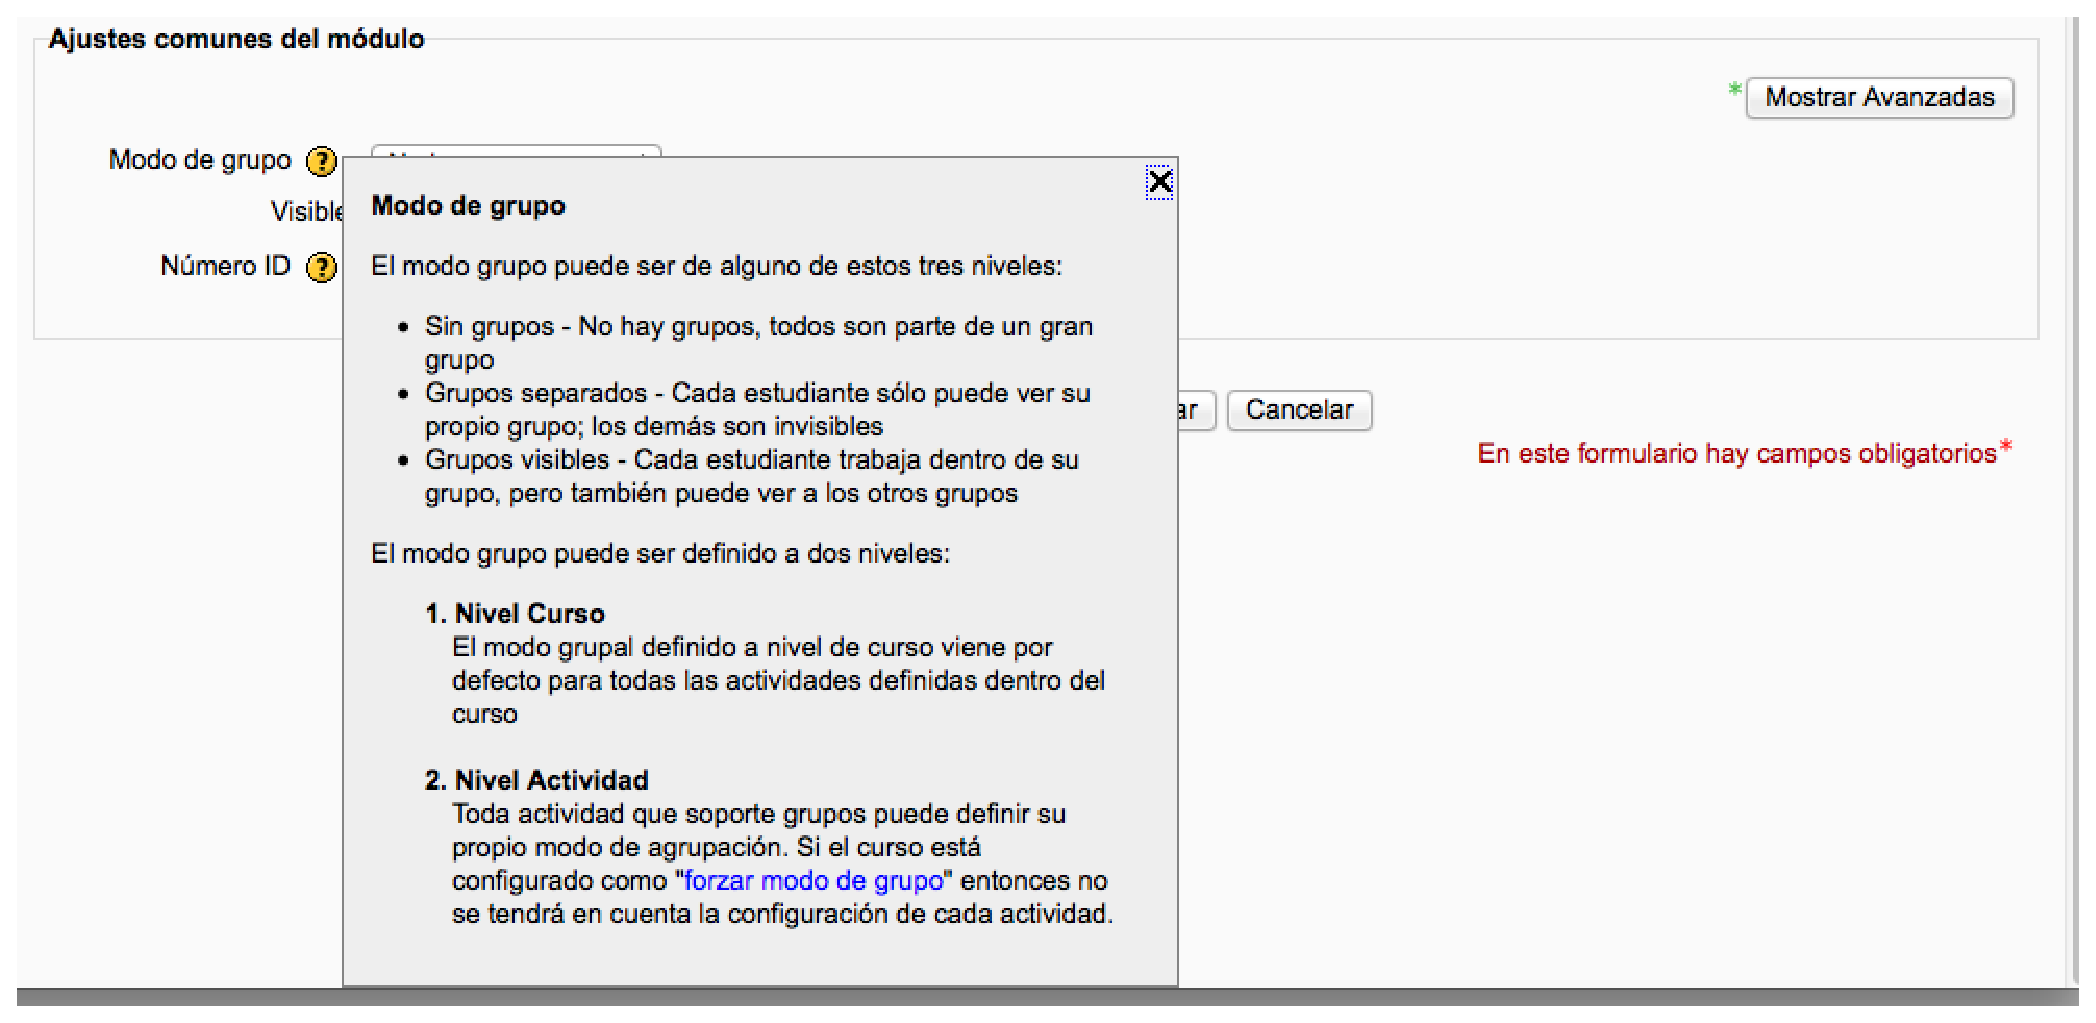
\includegraphics[width=0.7\textwidth]{./img/c4paramhelp.eps}
	\caption{Pantalla de ayuda a la configuración Wikicode}
\end{figure}

\newpage

\subsubsection{Pantalla cabecera superior}

Como su propio nombre indica, no se trata de un interfaz completo en sí, sino de la parte superior que compartirán todas las páginas definidas dentro del módulo Wikicode. Esta cabecera, compartida, la podemos dividir en las siguientes partes.

\begin{itemize}
	\item \textbf{Nombre del curso:} Etiqueta informativa sobre el nombre del curso al que pertenece la Wikicode.
	\item \textbf{Listado de navegación:} Menú de tipo lista que nos permite acceder al resto de contenidos del curso.
	\item \textbf{Árbol de directorio:} Nos representa un listado de donde nos encontramos ahora mismo, situándonos en el curso, la categoría y el nombre que hayamos dado al módulo. Será navegable y permite enlazar rápidamente a cada una de ellas.
	\item \textbf{Actualización:} Si el usuario tiene permisos de administración le aparecerá este botón, el cual permite acceder a la parametrización de la Wikicode que nos encontremos y modificar sus opciones.
	\item \textbf{Menú de contenido:} Menú de navegación que nos permite desplazarnos rápidamente por las opciones de nuestro editor de desarrollo. Se marcará la opción sobre la que nos encontremos en el momento.
\end{itemize}

En la siguiente figura se muestra la cabecera que se presentará en todas las opciones del módulo Wikicode:

\begin{figure}[h]
	\centering
	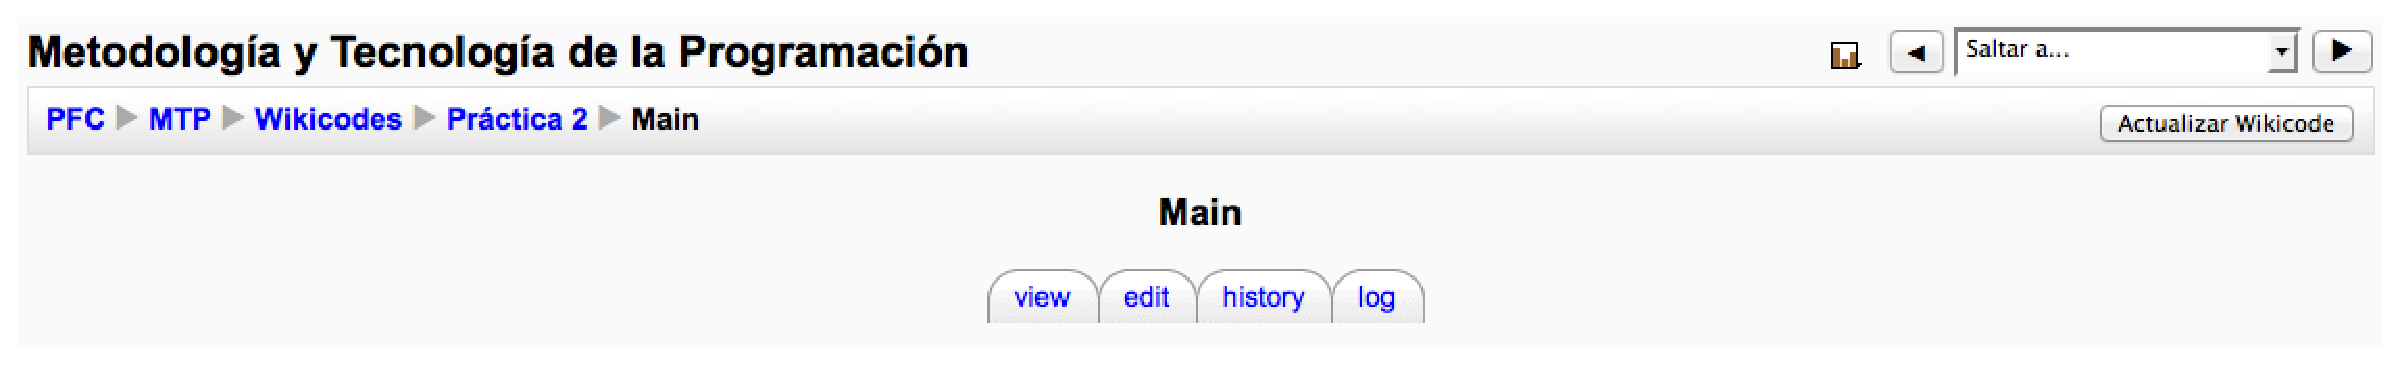
\includegraphics[width=\textwidth]{./img/c4menu.eps}
	\caption{Pantalla cabecera Wikicode}
\end{figure}

\newpage

\subsubsection{Pantalla visualización}

Se trata de la pantalla donde el usuario puede consultar, en formato texto plano, el código fuente de la Wikicode. La pantalla comparte el menú superior con el resto de opciones y simplemente nos mostrará esta información.

Sin embargo, para mayor utilidad de la misma, si el tutor ha decidido crear la Wikicode de modo grupal le aparecerá un menú donde podrá seleccionar el grupo que desee visualizar. Esta opción también será activa para los alumnos en caso de que el tutor así lo marcara.

En la siguiente figura se muestra el formulario de visualización con la opción de selección de grupos activada:

\begin{figure}[h]
	\centering
	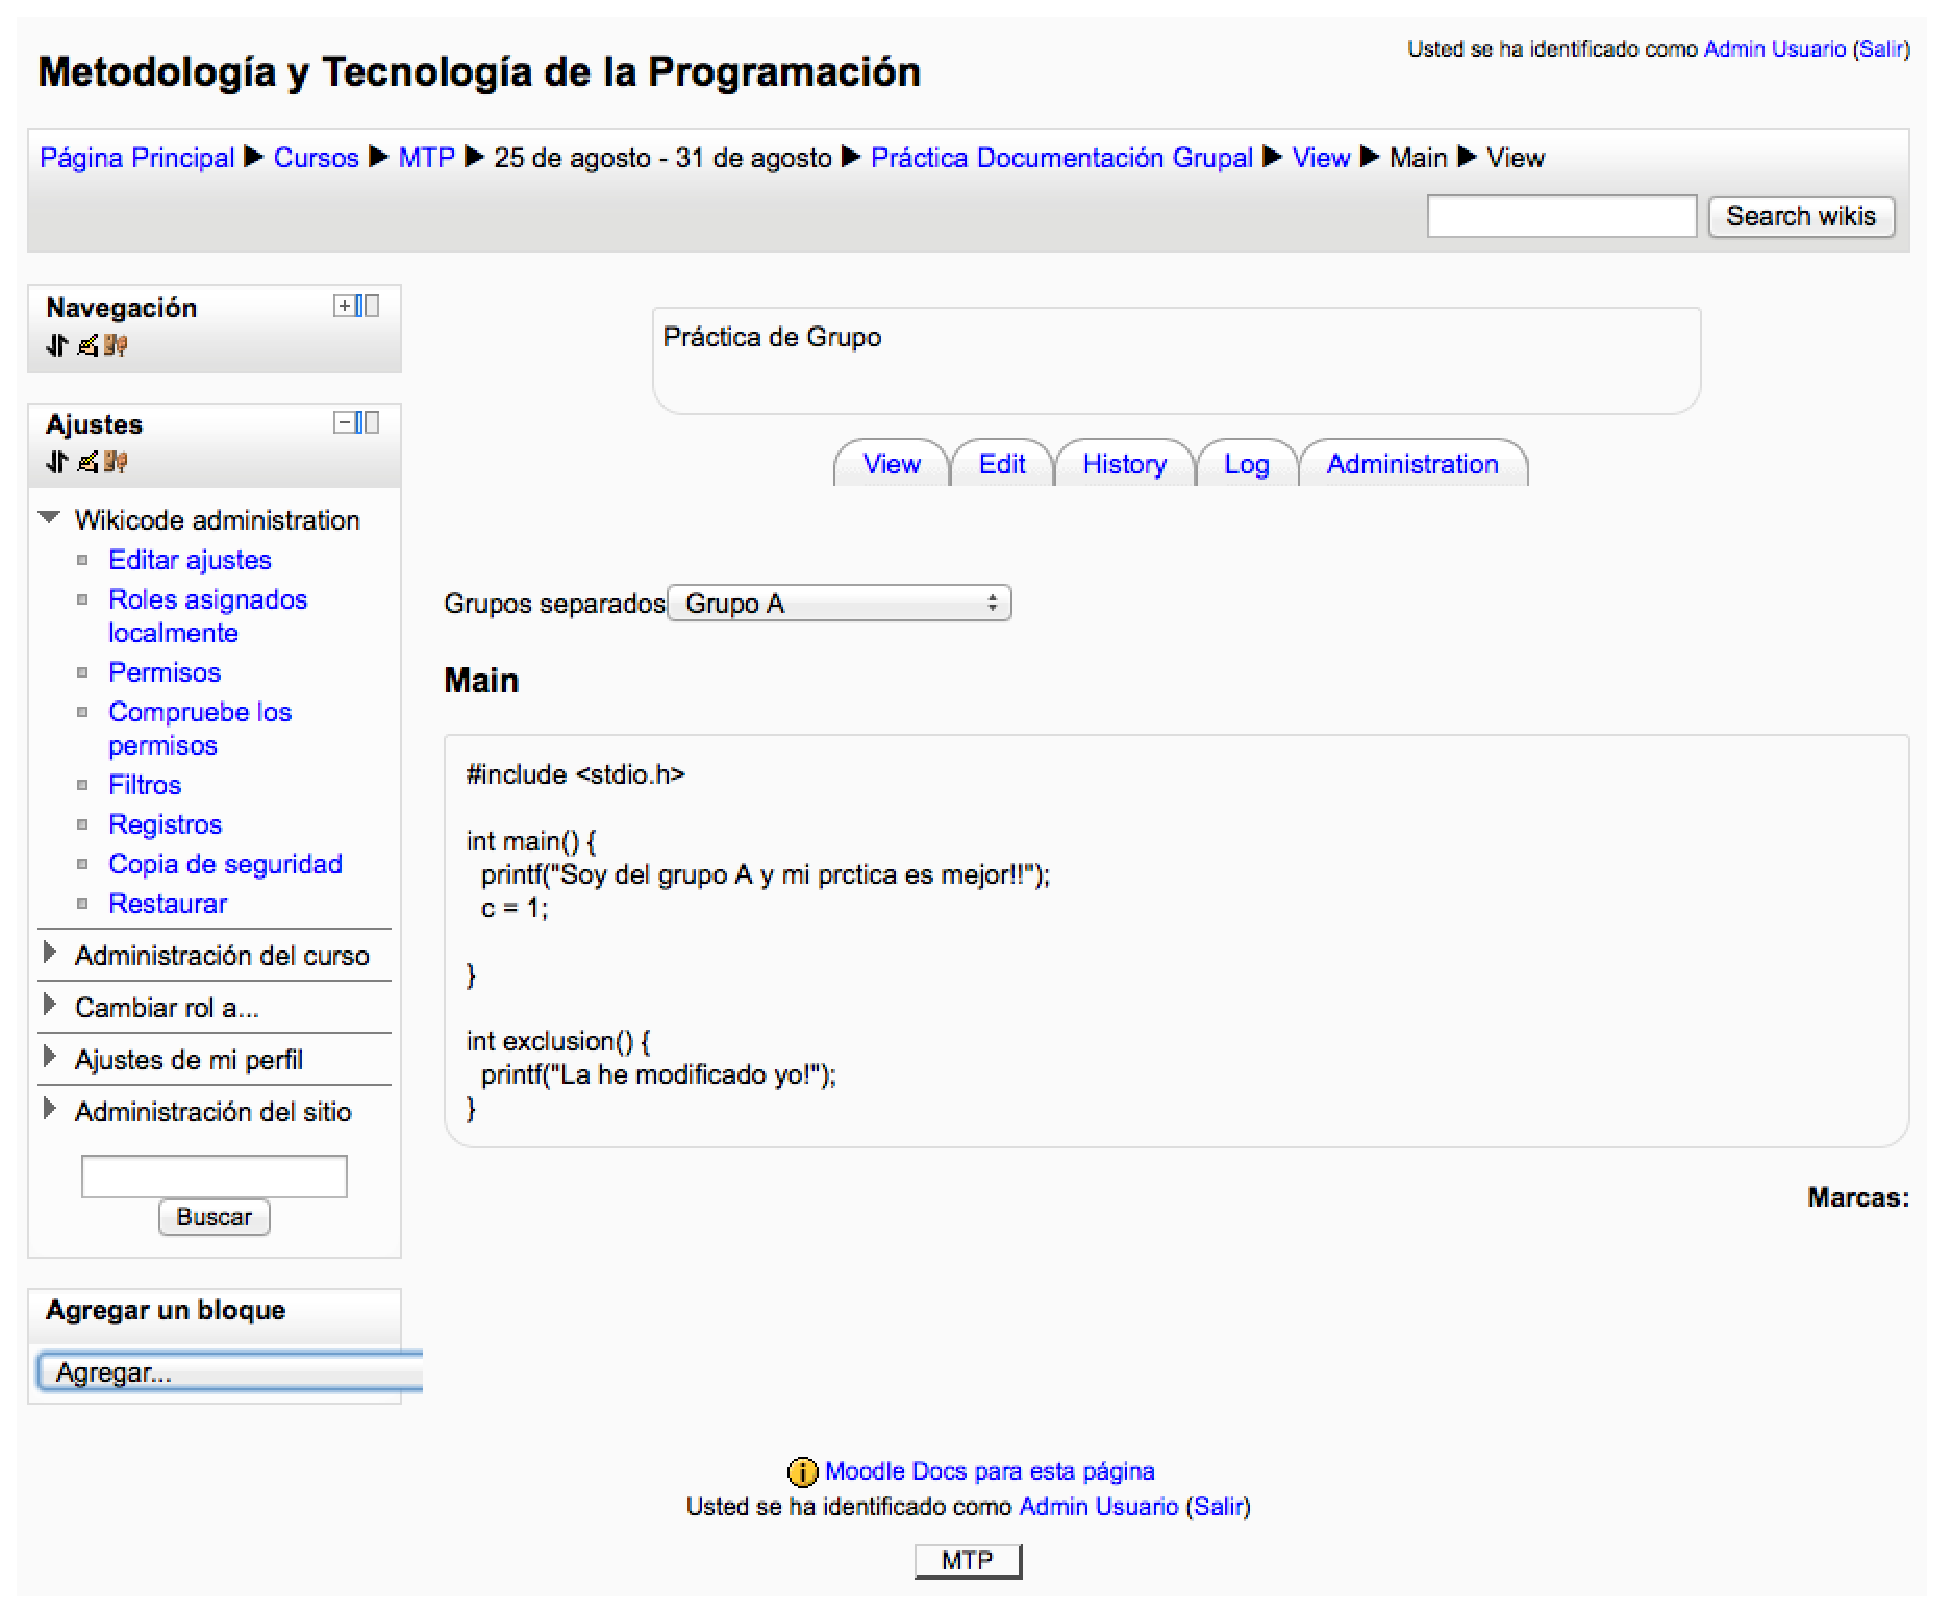
\includegraphics[width=\textwidth]{./img/c4view.eps}
	\caption{Pantalla visualización Wikicode}
\end{figure}

\newpage

\subsubsection{Pantalla edición}

Se trata de la pantalla clave del entorno de desarrollo, en la cual podremos editar el código fuente, comunicarnos con el resto de usuarios y compilar nuestro código para ver que errores puede contener.

\begin{figure}[h]
	\begin{center}
	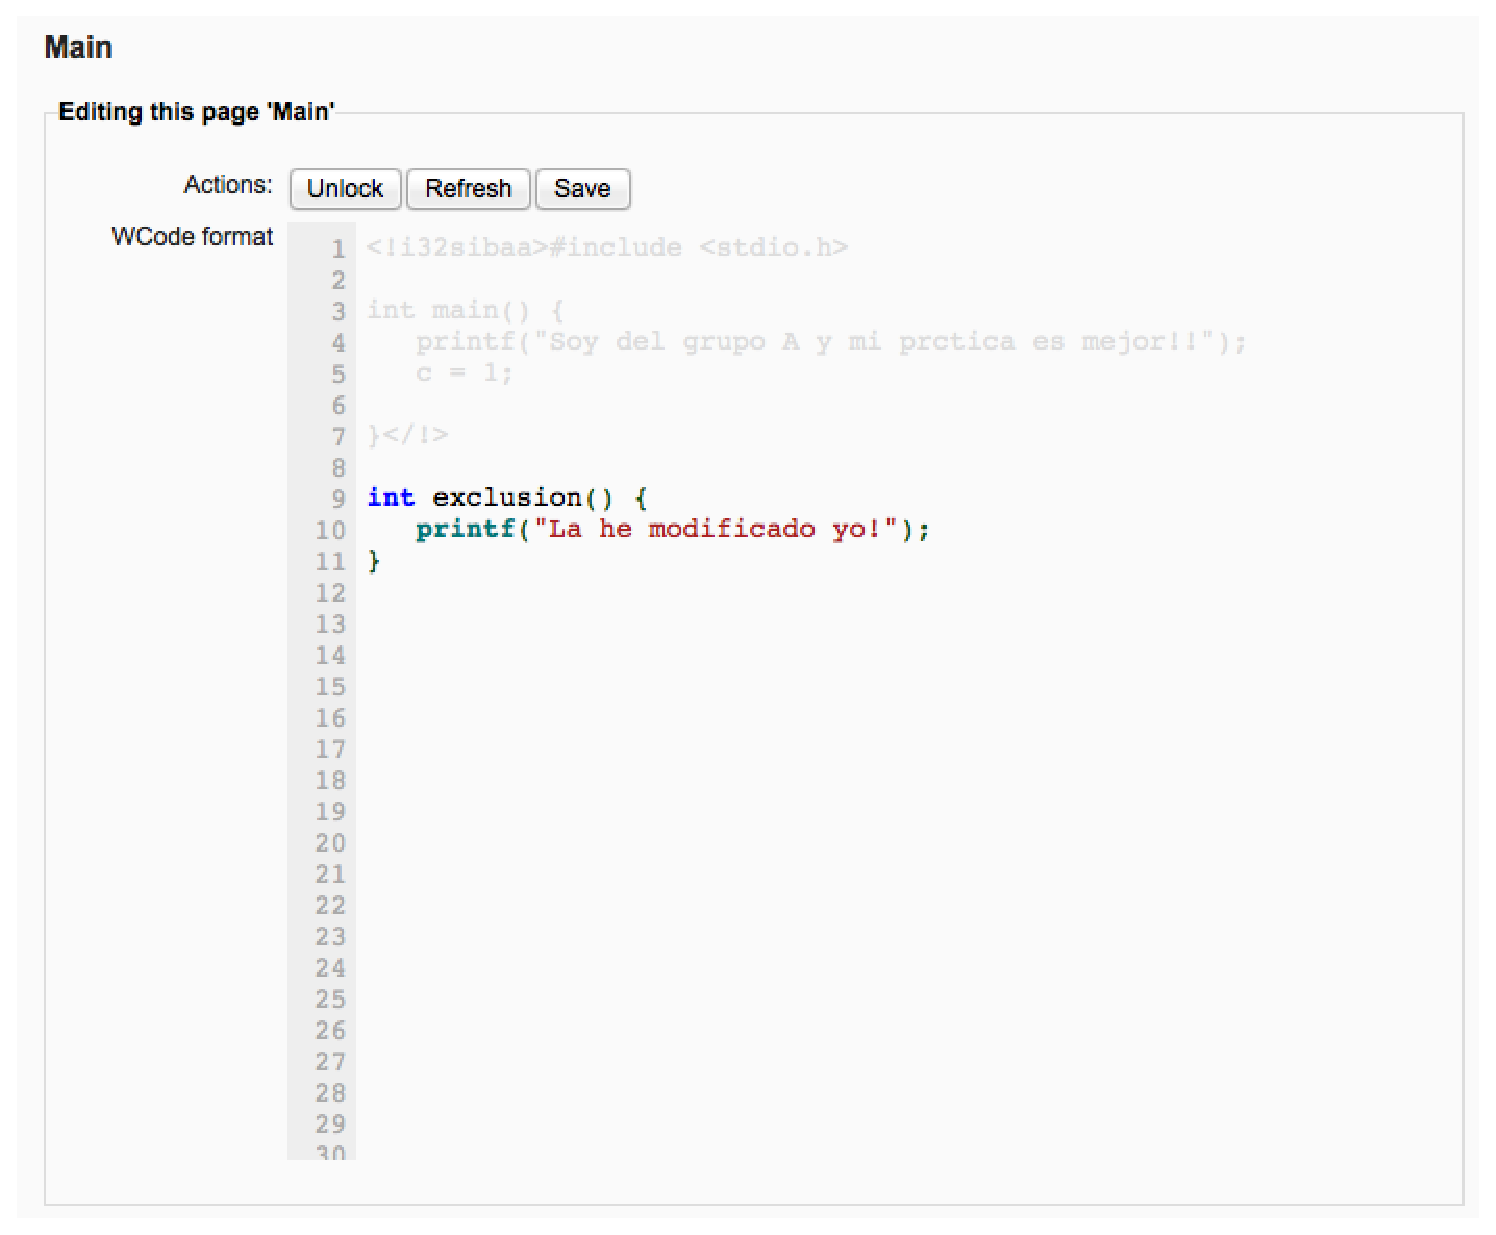
\includegraphics[width=\textwidth]{./img/c4edit.eps}
	\caption{Pantalla editor Wikicode.}
	\end{center}
\end{figure}

El editor de código se irá actualizando a medida que el usuario va escribiendo. Del mismo modo, si intentamos escribir en una parte del código bloqueada el editor nos impedirá esa acción. Las partes bloqueadas por otros usuarios están claramente diferenciadas en otro color y a su vez se nos informa que usuario es el dueño de dicha parte.

Para comodidad del usuario final, se da formato y color al código conforme a los estándares en C siguiendo este estilo:

\begin{description}
	\item[Comentarios]: Color marrón [\#BB9977]
	\item[Palabra clave]: Color azul y tipografía en negrita.
	\item[Cadena]: Color burdeos [\#AA2222]
	\item[Números]: Color verde claro [\#3A3]
	\item[Funciones]: Color turquesa [\#077] y tipografía en negrita.
	\item[Definición]: Color verde oscuro.
	\item[Bloqueo]: Color gris claro.
\end{description}

Los botones de la parte superior de este apartado actúan del siguiente modo:

\begin{description}
	\item[Unlock]: Nos abre una ventana de estilo pop-up que nos permite desbloquear las funciones que tengamos bloqueadas del código. Podemos elegir entre una, varias o todas.

\begin{figure}[h]
	\begin{center}
	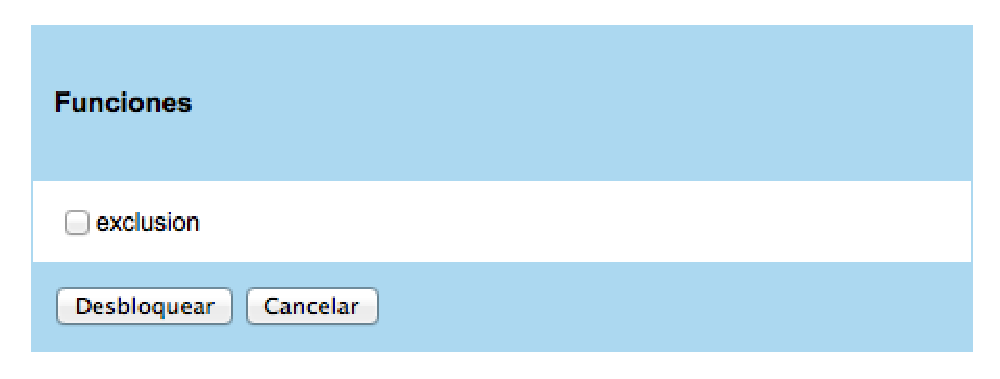
\includegraphics[width=0.5\textwidth]{./img/c4unlock.eps}
	\caption{Pantalla desbloqueo Wikicode.}
	\end{center}
\end{figure}
	
	\item[Refresh]: Actualiza el código fuente. La actualización es semi-automática, pero si se requiere se puede efectuar esta operación manualmente.
	\item[Save]: Guarda una copia del código fuente en el histórico y desbloquea todas las funciones.
\end{description}

Para comunicarnos con otros usuarios se ha creado un chat, el cual se dividirá en dos partes. La superior mostrará los mensajes que han sido enviados con anterioridad, informándonos del usuario y la hora a la que se envió este mensaje. En la inferior habrá un campo de texto y un botón de envío, los cuales servirán para añadir nueva información al chat.

El diseño de este elemento del formulario se puede contemplar en la siguiente figura:

\begin{figure}[h]
	\begin{center}
	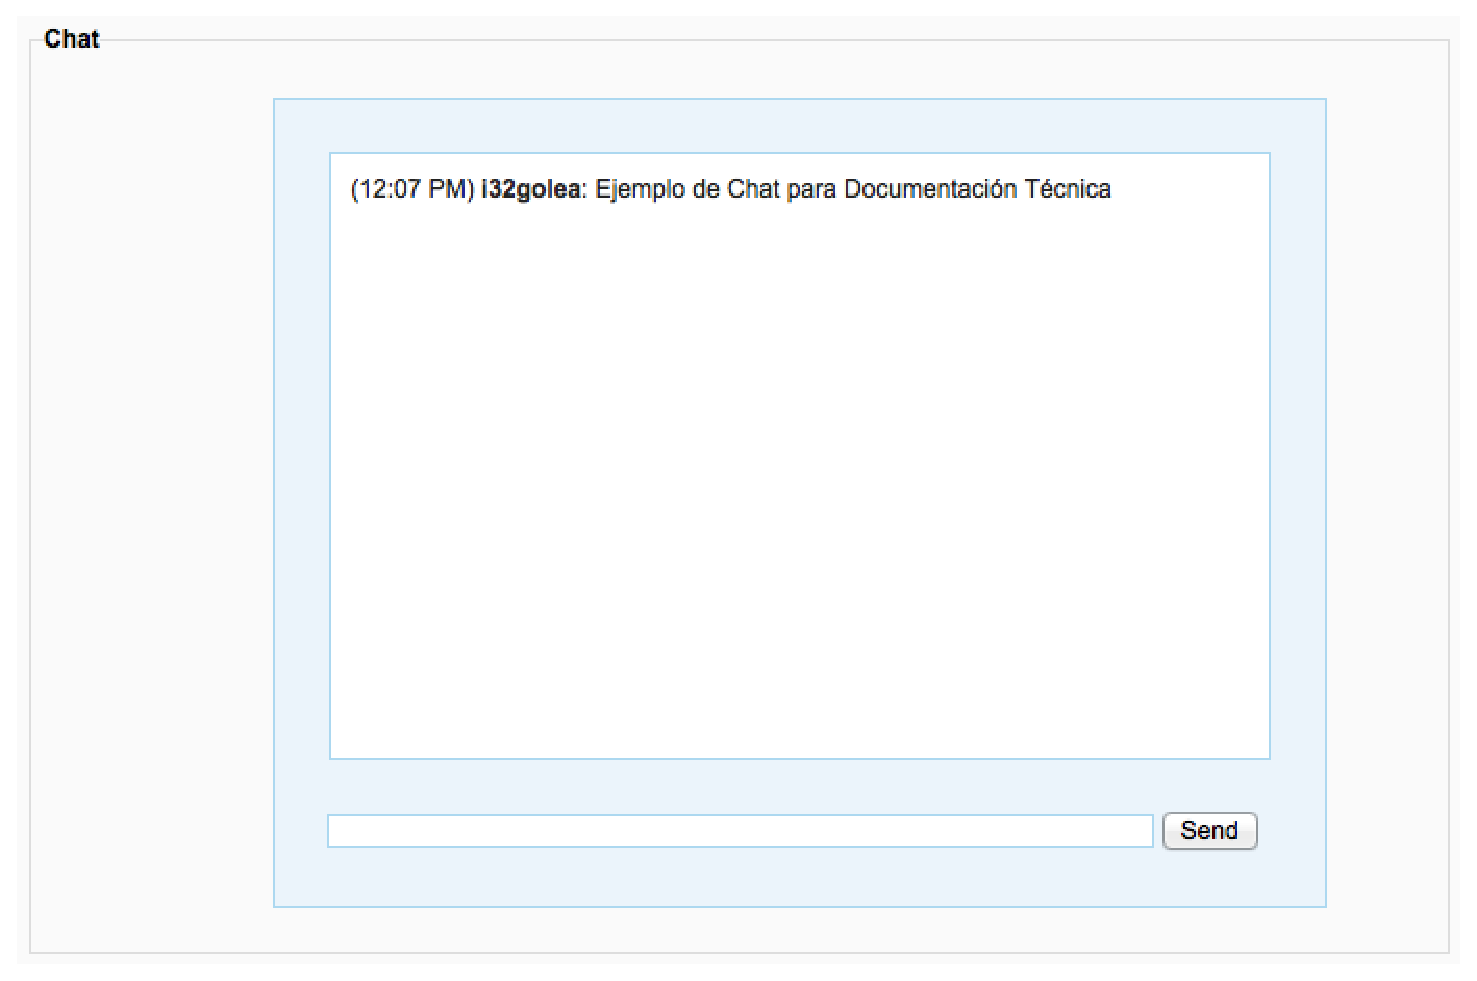
\includegraphics[width=0.65\textwidth]{./img/c4chat.eps}
	\caption{Pantalla chat Wikicode.}
	\end{center}
\end{figure}

Como última parte de este formulario vamos a diseñar la parte dedicada a la compilación, la cual estará dividida en dos partes:

\begin{itemize}
	\item Mensaje: Es el resultado de nuestra compilación, en la que se informará con un mensaje si se ha podido compilar de modo correcto y se nos informará de los errores en caso de que esta premisa no se cumpla. En ella se nos informará del error cometido y se nos proporcionará una pequeña ayuda para solucionarlo.
	\item Botones: Se tratarán de dos botones que nos permitirán dos acciones parejas. En la primera se llamará al compilador para obtener la información sobre nuestro código fuente. La segunda es una ampliación de la primera, la cual llamará al compilador y, si todo es correcto, nos permitirá descargar un ejecutable para ejecutarlo en el equipo cliente.
\end{itemize}

El diseño de este elemento se encuentra en la siguiente figura:

\begin{figure}[h]
	\begin{center}
	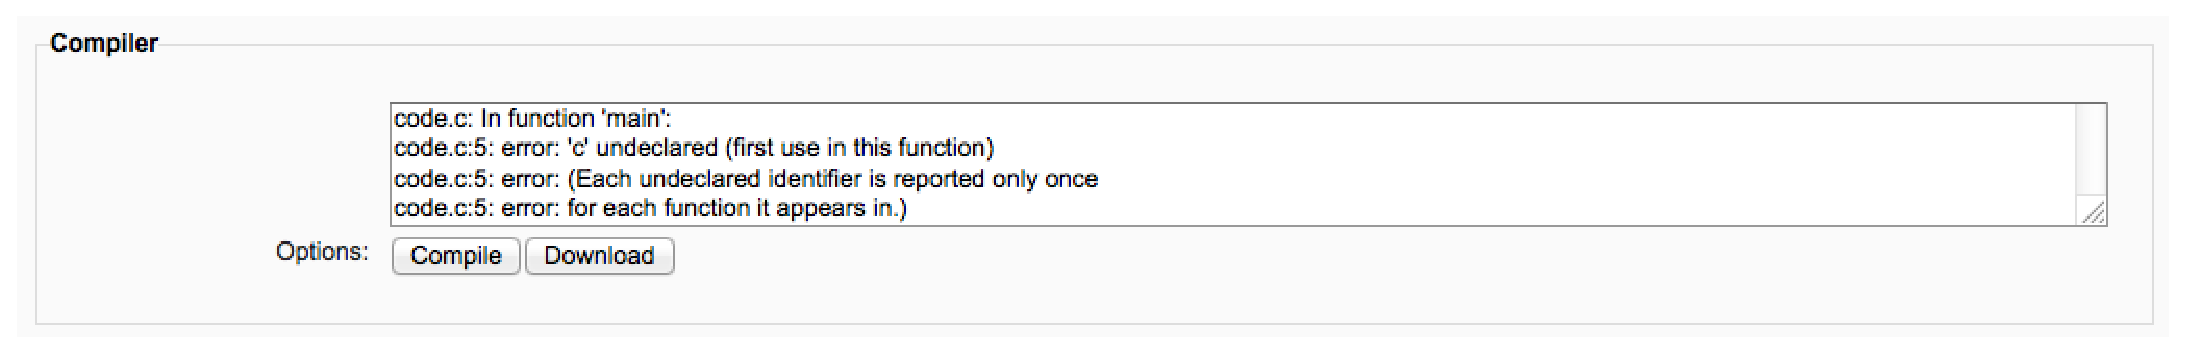
\includegraphics[width=\textwidth]{./img/c4compile.eps}
	\caption{Pantalla compilación Wikicode.}
	\end{center}
\end{figure}

\newpage

\subsubsection{Pantalla histórico}

Como su propio nombre indica, se trata del interfaz que vamos a utilizar para consultar las versiones anteriores de un código fuente. Se proporcionará una lista de versiones y se creará una tabla informando de quién creó dicha versión y cuando la creó.

\begin{figure}[h]
	\begin{center}
	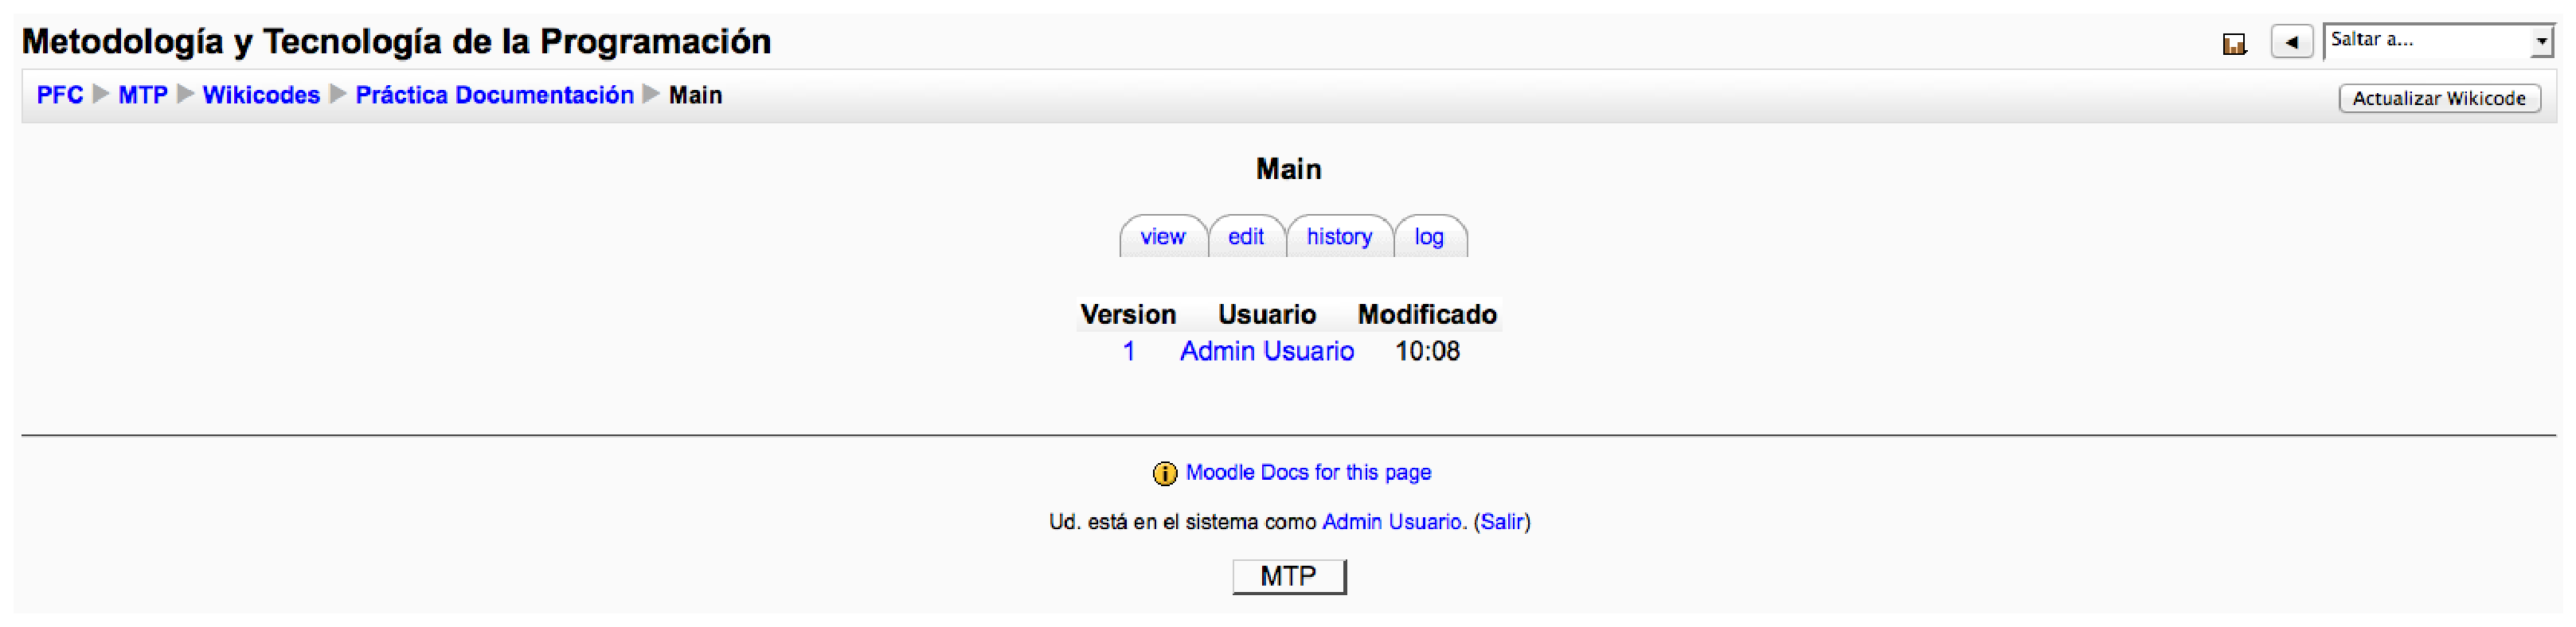
\includegraphics[width=\textwidth]{./img/c4history1.eps}
	\caption{Pantalla histórico Wikicode.}
	\end{center}
\end{figure}

Una vez pulsemos encima de una de estas versiones que se nos ofrece, podremos visualizar el código fuente que había en tal fecha y restaurarlo si así lo vemos oportuno pulsando el enlace a la izquierda de la pantalla. Dicho enlace nos llevará a otro formulario donde se nos pedirá autorización para realizar dicha acción.

\begin{figure}[h]
	\begin{center}
	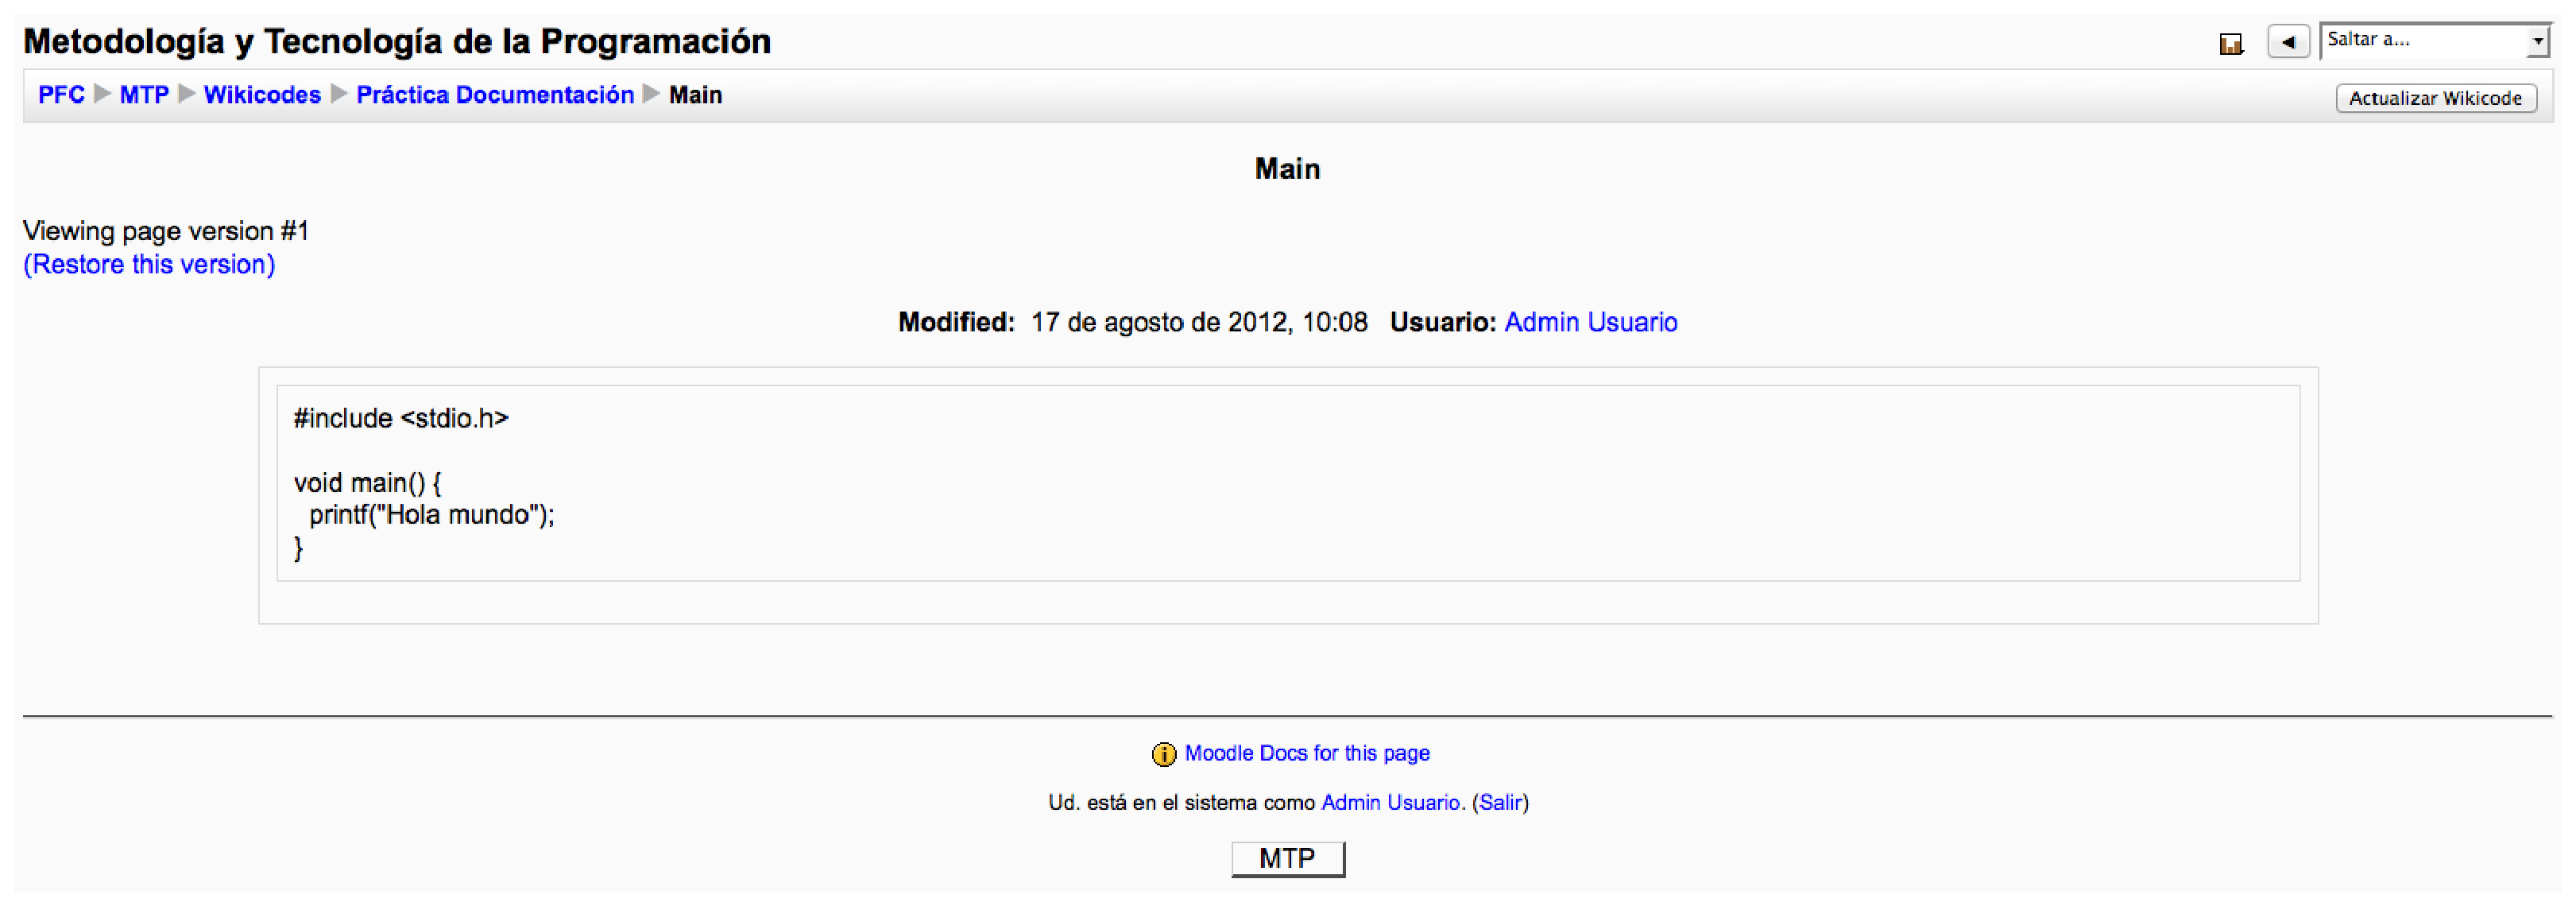
\includegraphics[width=\textwidth]{./img/c4history2.eps}
	\caption{Pantalla restauración histórico Wikicode.}
	\end{center}
\end{figure}

Una de las mayores novedades que presenta el módulo para la versión 2 de Moodle es la inclusión de una potente herramienta que nos permite comparar dos códigos, señalando en el propio interfaz las diferencias entre ambos. El diseño de dicha herramienta se puede ver en la siguiente figura, y para llamarlo habrá que seleccionar dos versiones en la Figura 4.12 y pulsar el botón denominado``Comparar''.

\begin{figure}[h]
	\begin{center}
	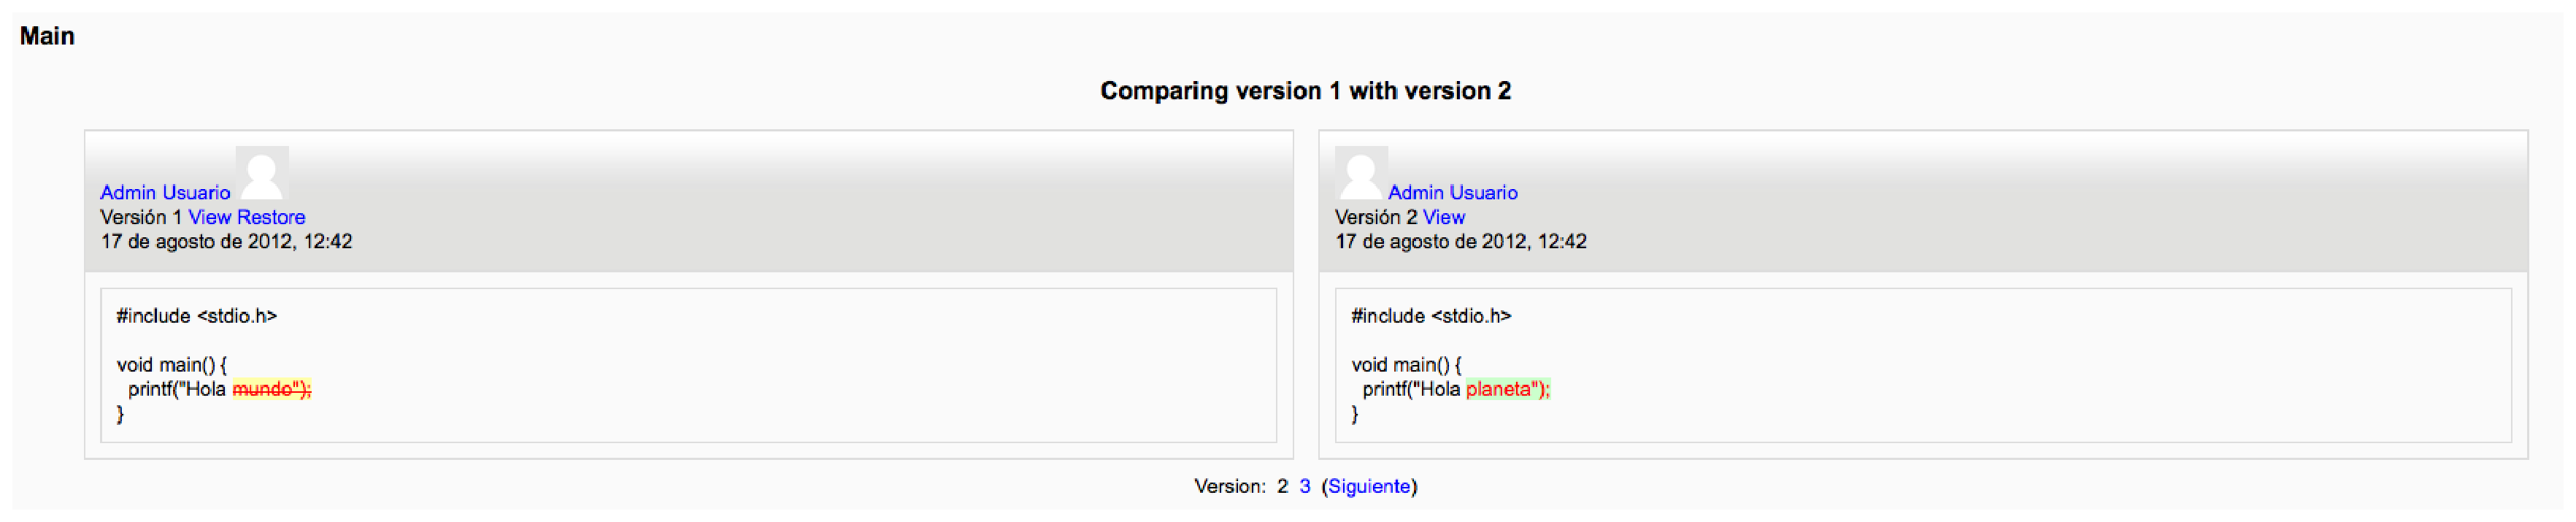
\includegraphics[width=\textwidth]{./img/c4diff.eps}
	\caption{Pantalla comparación histórico Wikicode.}
	\end{center}
\end{figure}

\subsubsection{Pantalla estadísticas}

Este formulario, el último a diseñar, es el que se encargará de traernos la información estadística almacenada en base de datos con respecto al código fuente. Se accede a él pulsando el botón log del menú superior, y una vez dentro de él nos encontraremos una serie de etiquetas con un campo de texto informándonos de su resultado.

Como novedad, a partir de la versión 2 de Moodle se añaden unos botones de ayuda para explicar el significado de cada estadística. El diseño de dicho formulario se puede contemplar en la siguiente figura:

\begin{figure}[h]
	\begin{center}
	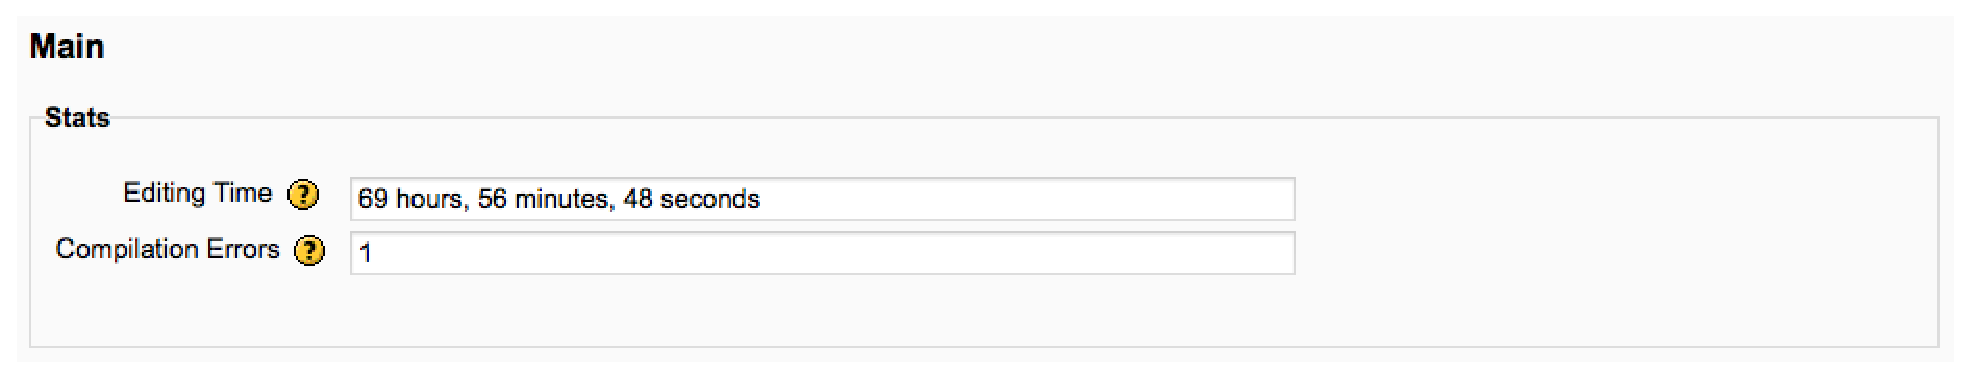
\includegraphics[width=\textwidth]{./img/c4log.eps}
	\caption{Pantalla estadística Wikicode.}
	\end{center}
\end{figure}

\section{Especificación procedimental}

Llegados a este punto, trataremos de modelar el módulo viendo sus aspectos dinámicos desde un alto nivel de abstracción, es decir, nos centraremos en las actividades de negocio más importantes en el dominio del problema. Para ello no pretendemos describir en detalle los procedimientos u operaciones que tienen lugar entre dichos objetos ni los atributos que se intercambian entre sí sino simplemente mostrar las actividades que tienen lugar entre ellos. Para ello, en los siguientes apartados comentaremos los diferentes diagramas de actividades asociados a cada una de los bloques explicados anteriormente.

\subsection{Diagrama de actividades para el sistema Wikicode-Mod}

\subsubsection{Actividad: Crear, configurar y parametrizar la Wikicode}

Una de las principales actividades que debe realizar el \emph{sistema Wikicode-Mod} es la creación de la actividad dentro de Moodle, así como configurarse correctamente para poder usarse en un futuro.

En la siguiente figura se muestra el diagrama de actividades asociado:

\begin{figure}[h]
	\centering
	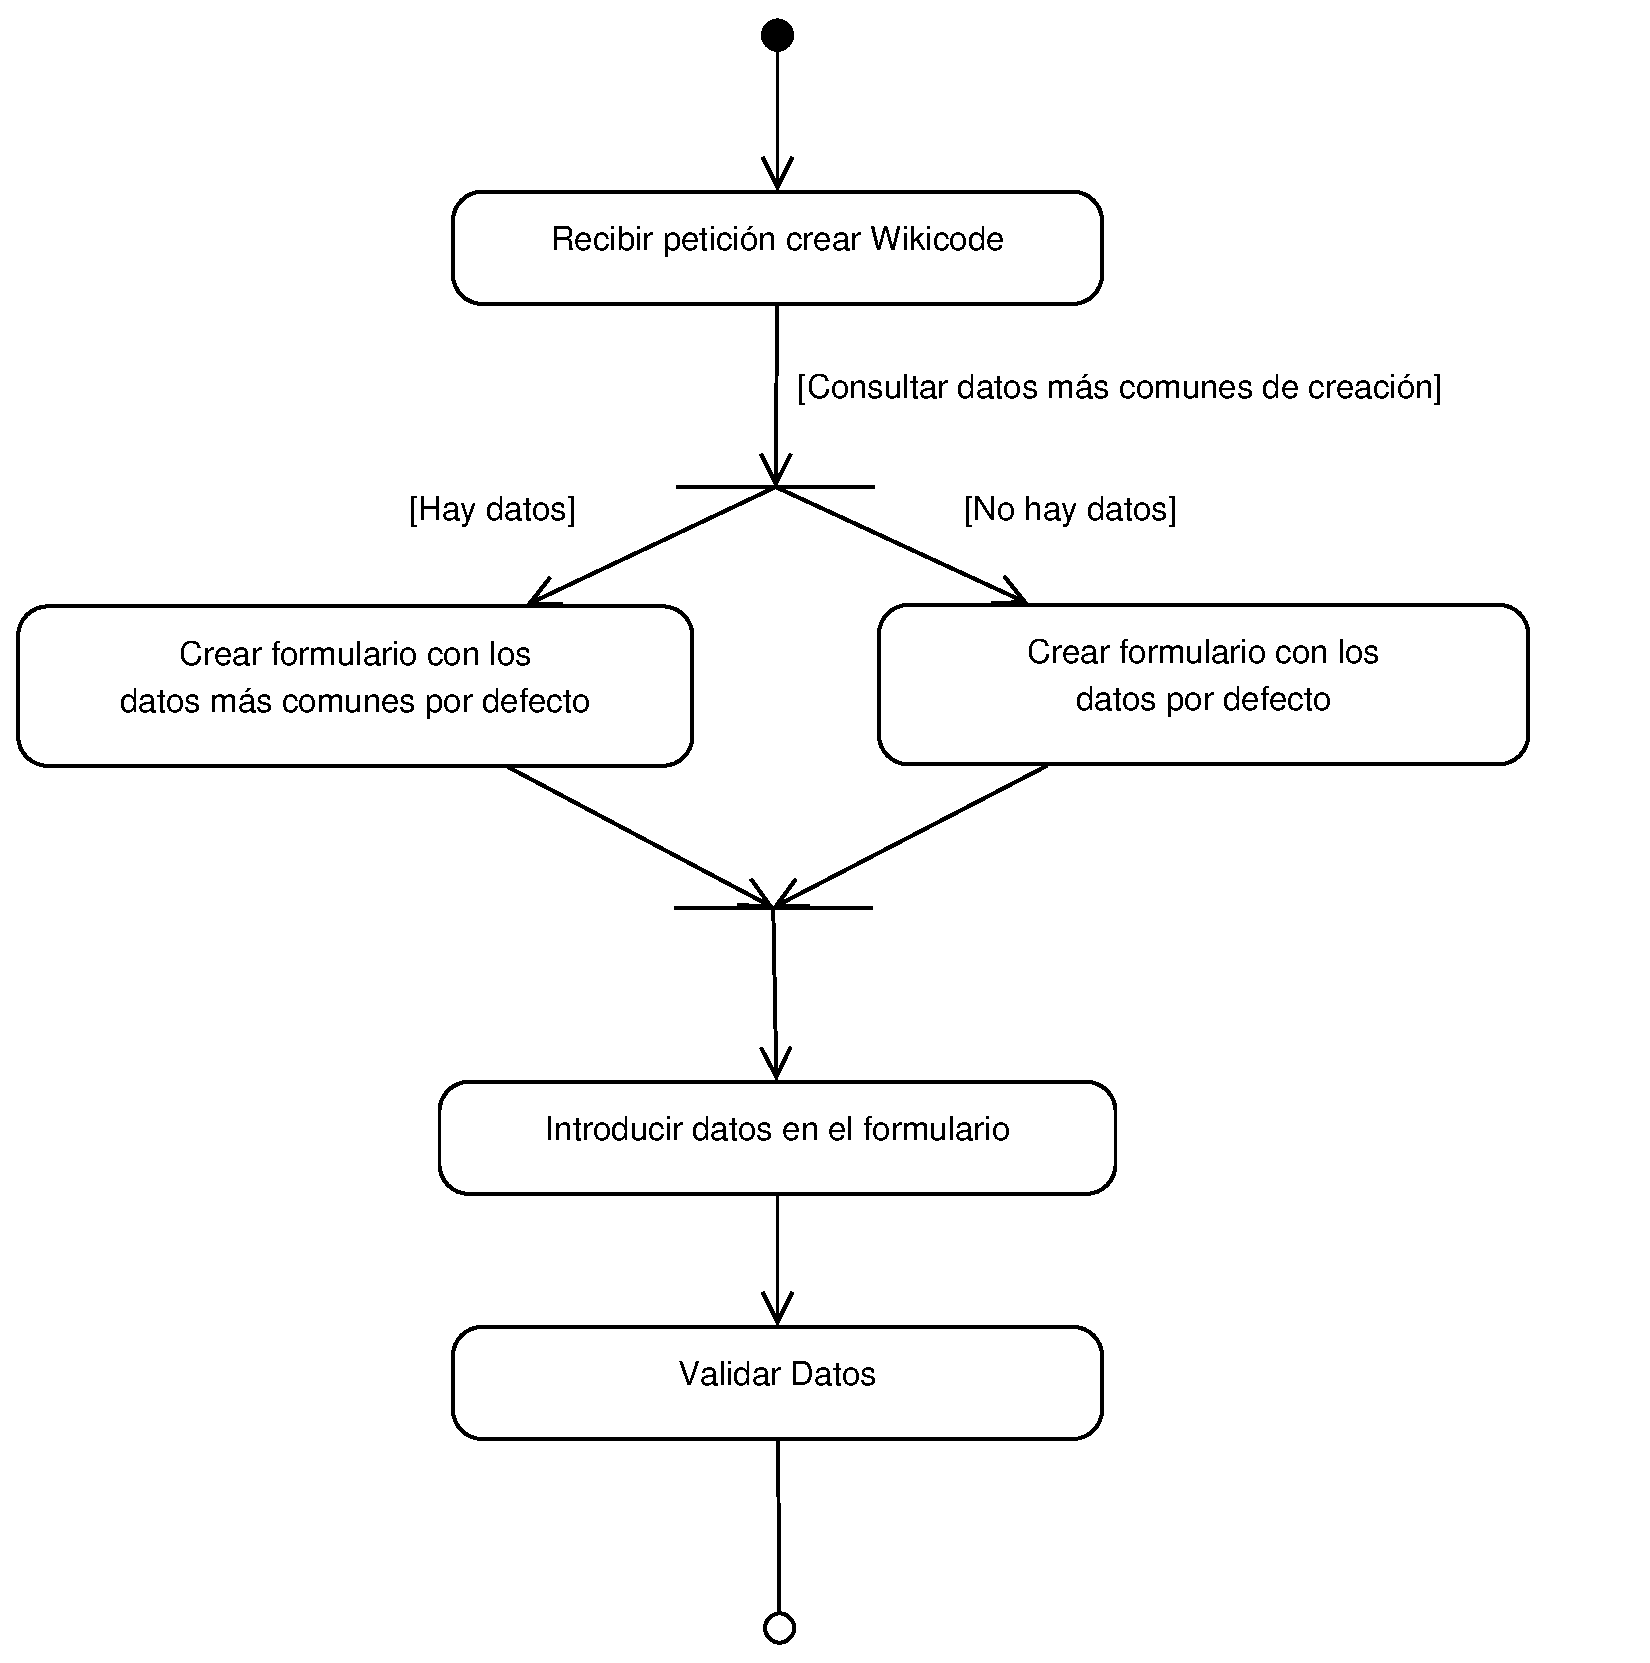
\includegraphics[width=0.7\textwidth]{./img/DiagramaA1.eps}
	\caption{Actividad crear, configurar y parametrizar la Wikicode}
\end{figure}

\newpage
\subsubsection{Actividad: Visualizar código fuente}

Es otra de las actividades que realiza el \emph{sistema Wikicode-Mod}. Se trata de una actividad muy simple en la que se muestra el código fuente de la Wikicode.

El diagrama de actividad es:

\begin{figure}[h]
	\centering
	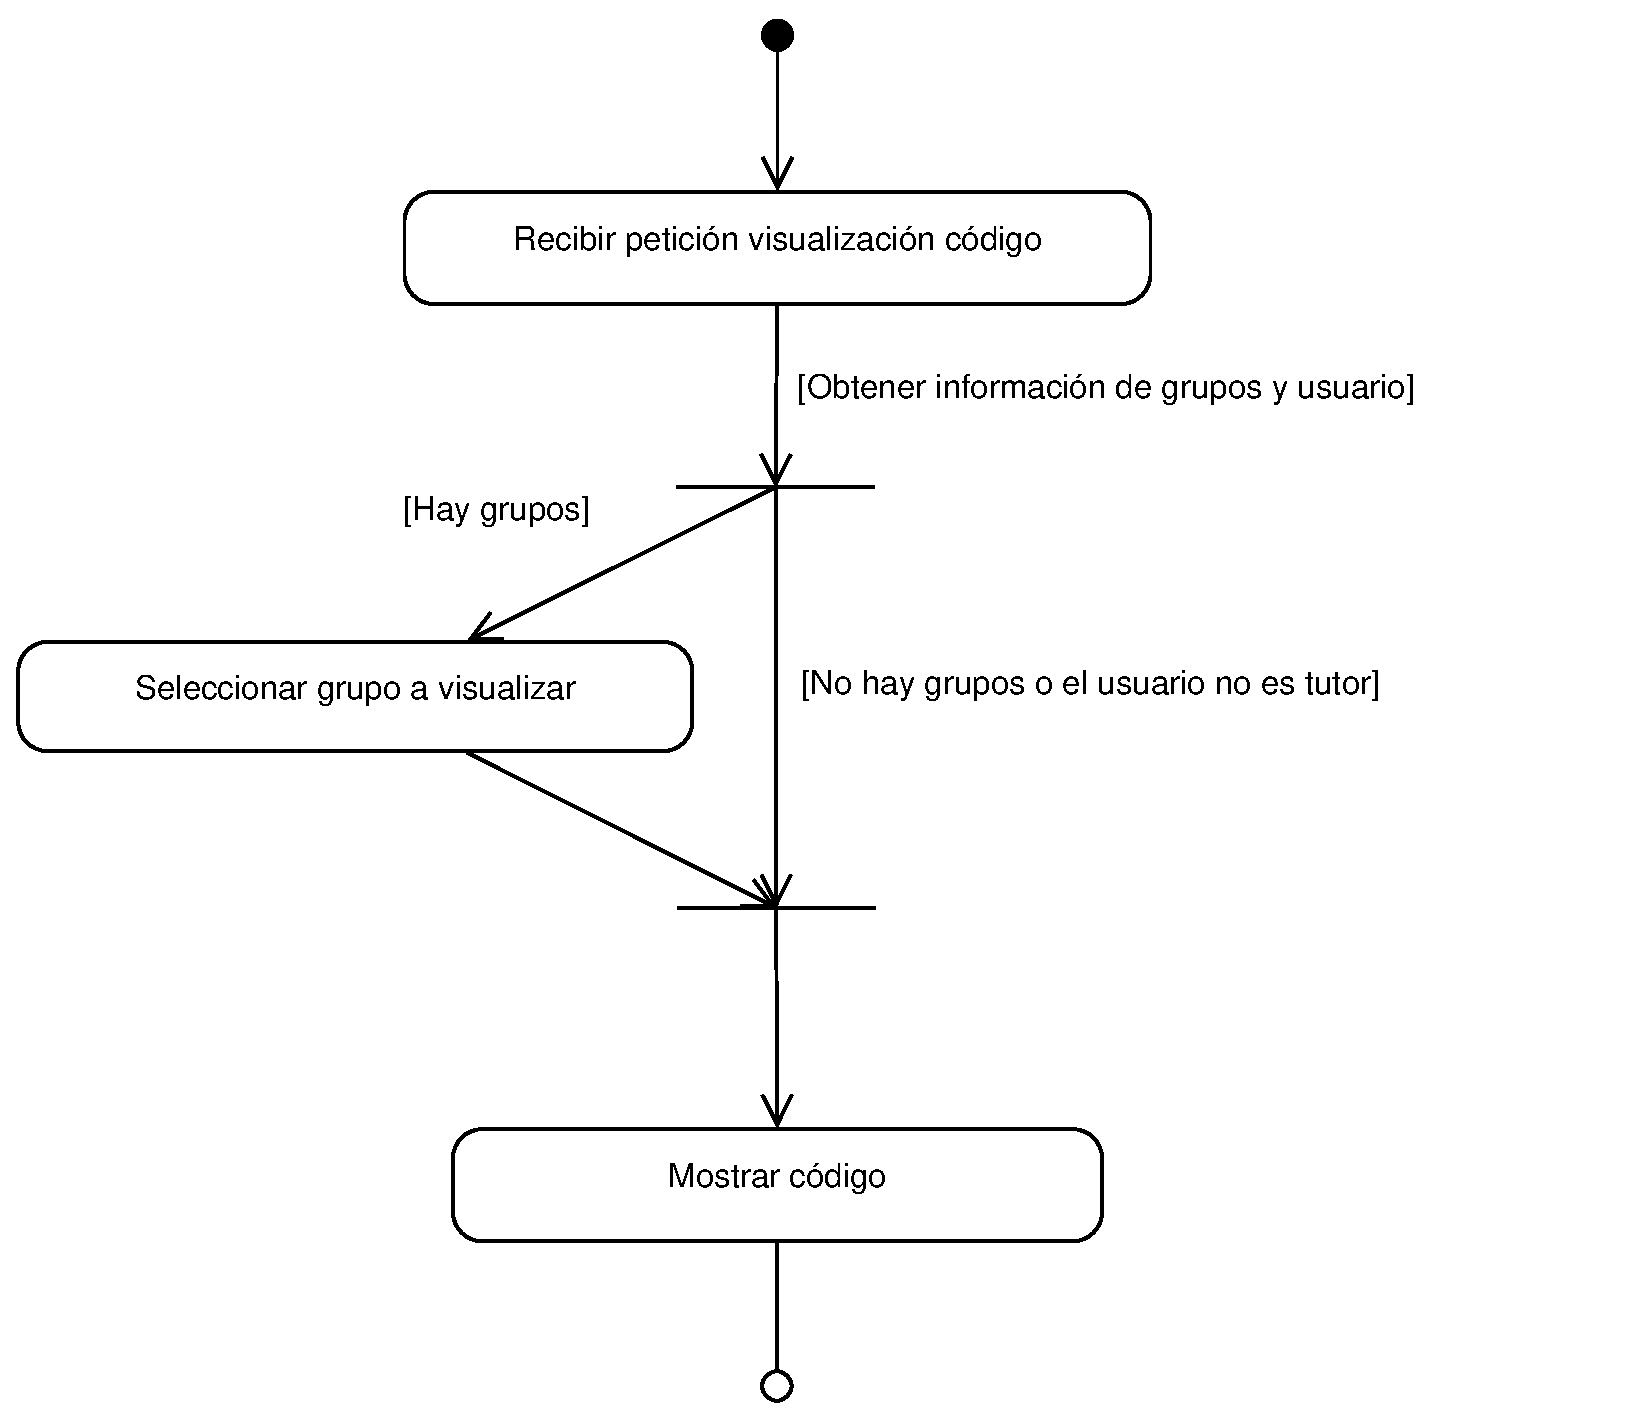
\includegraphics[width=0.7\textwidth]{./img/DiagramaA2.eps}
	\caption{Actividad visualizar código fuente}
\end{figure}

\subsubsection{Actividad: Editar código fuente}

La actividad que nos concierne en este subapartado se trata de la principal labor del \emph{sistema Wikicode-Mod}. Se trata de toda la actividad relacionada con la edición del código fuente, y cómo se almacena en base de datos de manera abstracta al usuario. Las teclas claves están definidas en la especificación de requisitos y la actividad de sincronización se explicará posteriormente.

\newpage

El diagrama de actividad es:

\begin{figure}[h]
	\centering
	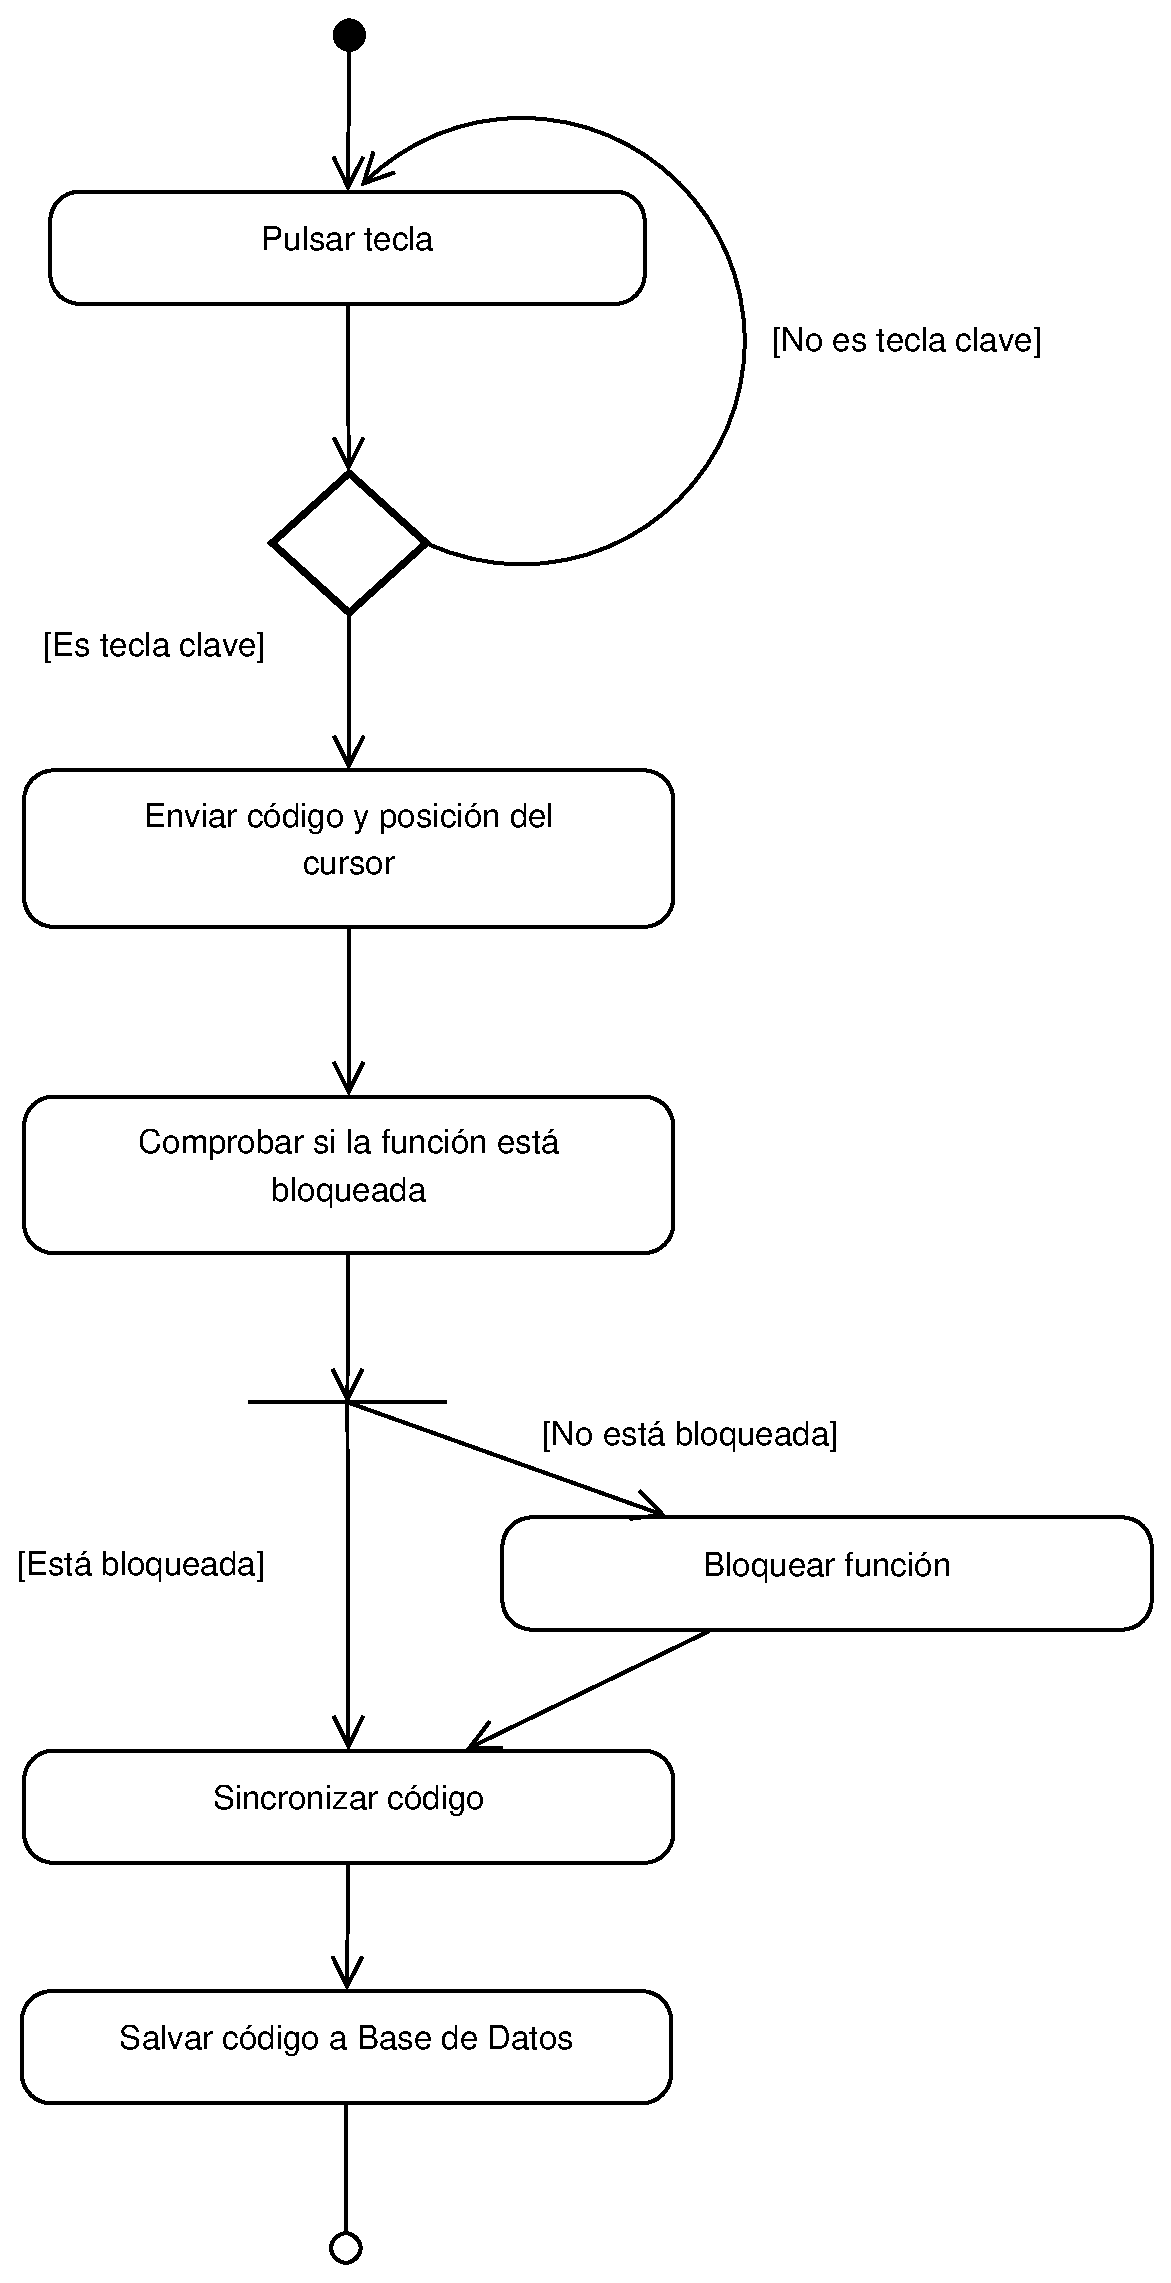
\includegraphics[width=0.54\textwidth]{./img/DiagramaA3.eps}
	\caption{Actividad editar código fuente}
\end{figure}

\newpage

\subsubsection{Actividad: Chat}

El chat es la siguiente actividad que vamos a describir, y es el módulo que utiliza el \emph{sistema Wikicode-Mod} para comunicar a los usuarios entre sí mientras están modificando un código fuente. Es una actividad secuencial en la que únicamente hay que escribir y leer un fichero en un intervalo de tiempo.

En la siguiente figura podemos comprobar el diagrama de actividades asociado al envío de mensajes:

\begin{figure}[h]
	\centering
	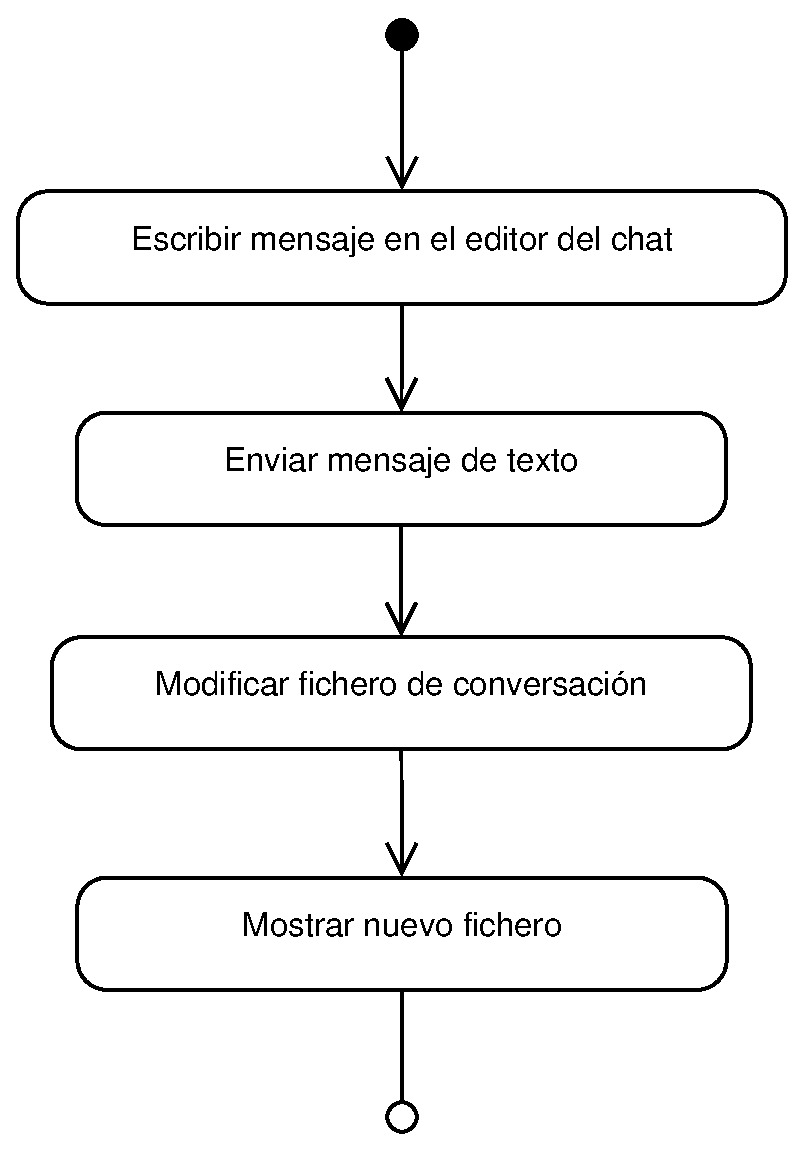
\includegraphics[width=0.4\textwidth]{./img/DiagramaA4.eps}
	\caption{Actividad chat}
\end{figure}

\newpage

\subsubsection{Actividad: Compilar código fuente}

La compilación es el proceso en el que un programa informático, conocido como compilador, traduce un programa escrito en un lenguaje de programación a otro que habitualmente suele ser el lenguaje máquina. En esta actividad el \emph{sistema Wikicode-Mod} tomará el código escrito en el editor y se lo pasará al compilador. Posteriormente podremos comprobar la respuesta de este.

El diagrama de actividad es el siguiente:

\begin{figure}[h]
	\centering
	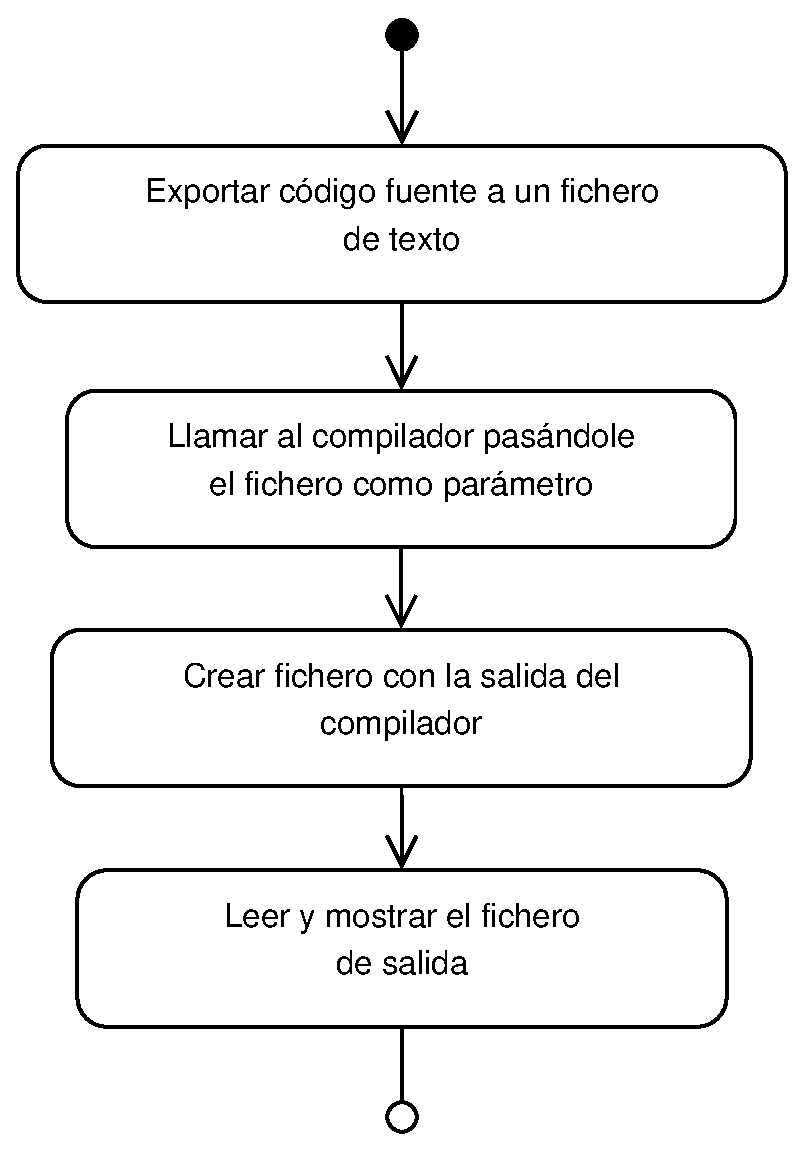
\includegraphics[width=0.4\textwidth]{./img/DiagramaA5.eps}
	\caption{Actividad compilar código fuente}
\end{figure}

\newpage
\subsubsection{Actividad: Visualizar histórico}

Es otra actividad que nos proporciona el \emph{sistema Wikicode-Mod}, en la cual podemos ir viendo toda la historia de un código fuente. Esto nos servirá para, en caso de que hayamos cometido un error, poder hacer un rollback a una versión antigua almacenada. En el histórico no se eliminará ninguna entrada, sino que la que hayamos seleccionado en caso de restauración se creará como una nueva versión. Es decir, sería similar a si hubiéramos copiado todo ese antiguo código y hubiéramos salvado.

Una vez restaurado, volveremos al editor y se podrá volver a editar.

El diagrama de actividad que nos proporciona esta actividad se muestra en la siguiente figura:

\begin{figure}[h]
	\centering
	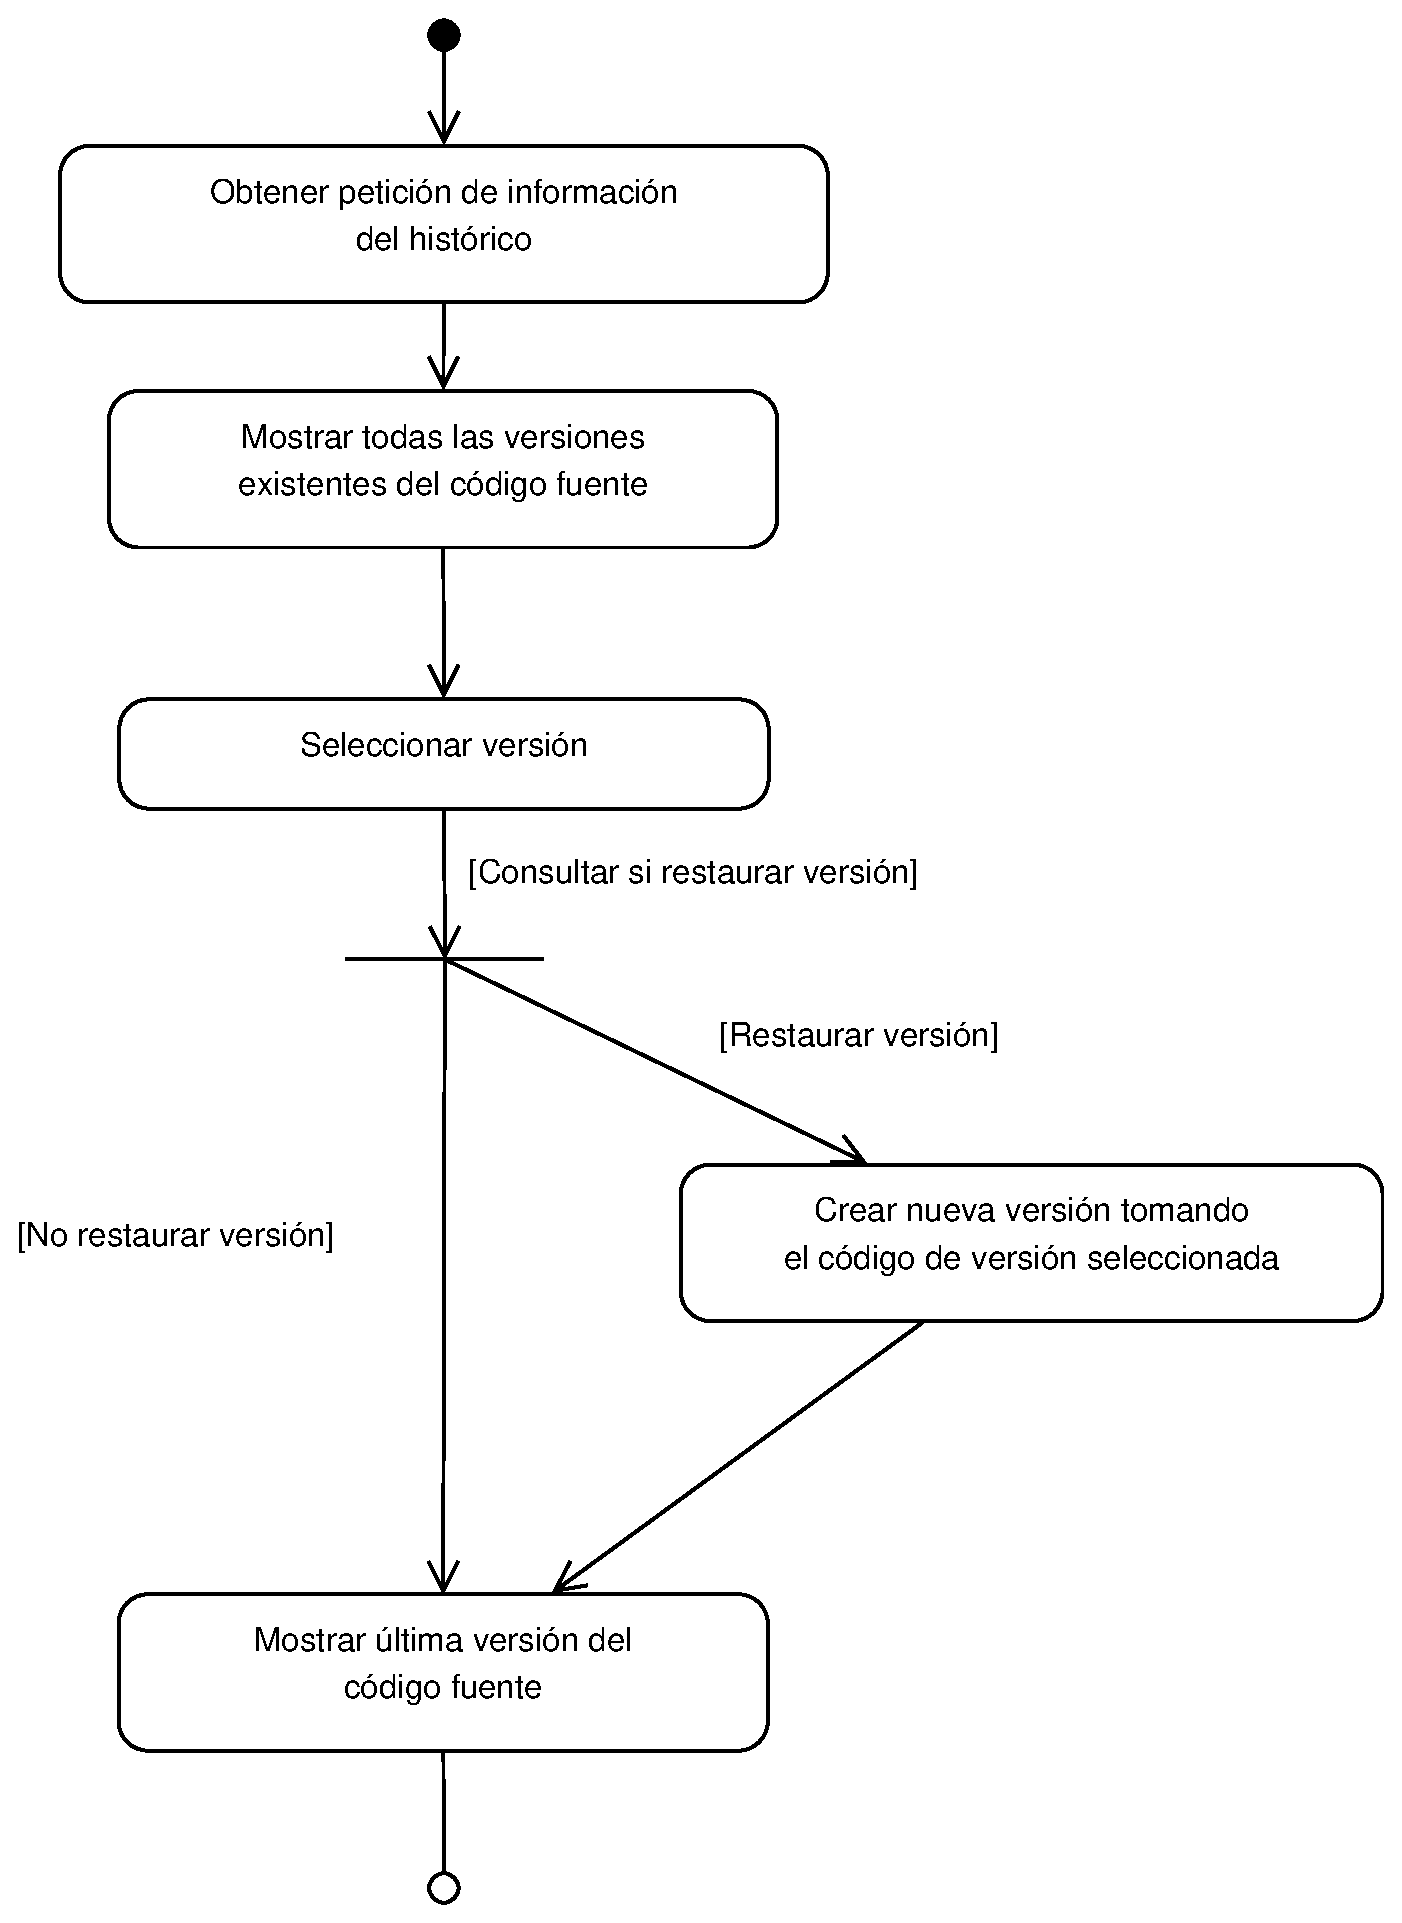
\includegraphics[width=0.6\textwidth]{./img/DiagramaA8.eps}
	\caption{Actividad visualizar histórico}
\end{figure}

\newpage
\subsubsection{Actividad: Visualizar estadísticas}

Es otra actividad del \emph{sistema Wikicode-Mod} puede ser una de las más utilizadas por los tutores para poder valorar la realización de prácticas de programación. En ella se puede consultar todo lo referente en torno a la programación de una actividad \emph{Wikicode} y se puede ampliar en un futuro con tantas estadísticas como se desee sin necesidad de variar el diagrama de actividad.

El diagrama de actividad se muestra en la siguiente figura:

\begin{figure}[h]
	\centering
	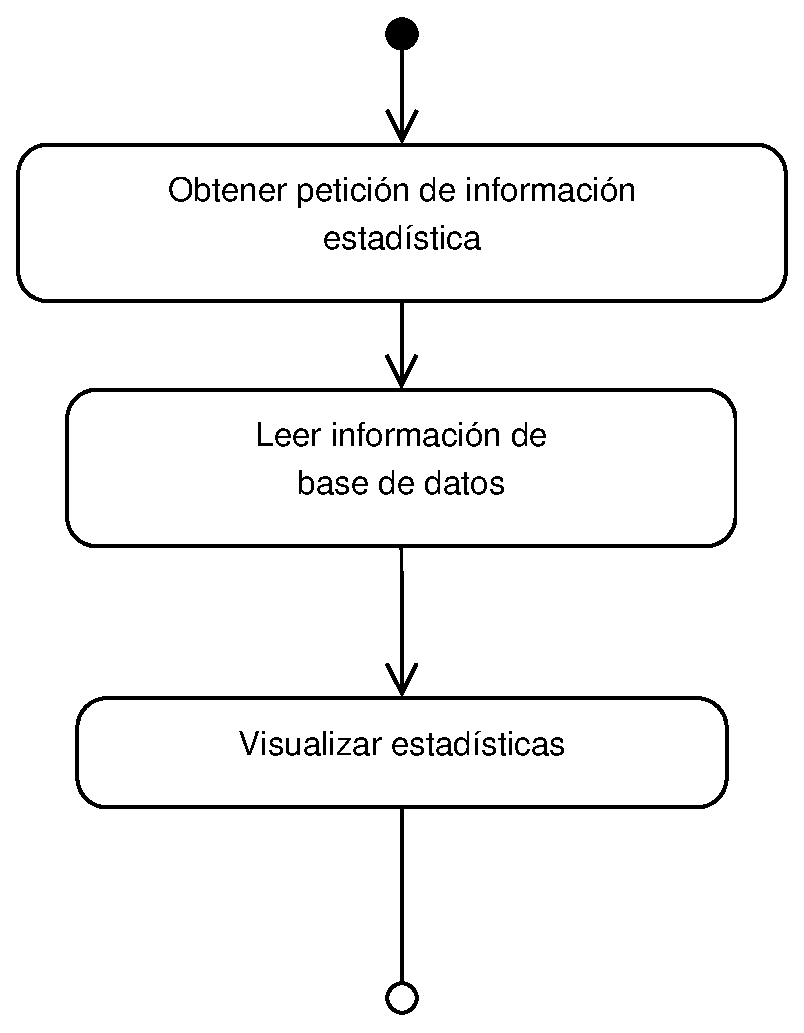
\includegraphics[width=0.5\textwidth]{./img/DiagramaA9.eps}
	\caption{Actividad visualizar estadísticas}
\end{figure}

\newpage
\subsection{Diagrama de actividades para el sistema Wikicode-Synchronizer}
\subsubsection{Actividad: Sincronizar código}

La sincronización de código es el procedimiento en el que se toma las variaciones del código fuente de un usuario y se pone en consonancia con el resto de usuarios. Del mismo modo, en ese mismo proceso se conseguirá tomar las variaciones de los otros usuarios para poder mostrárselo al usuario que está modificando su código. Así, se tratará de un proceso para poder ir viendo en tiempo real todas las modificaciones que va habiendo en un código sin necesidad de pisar el trabajo entre sí de los usuarios.

En la siguiente figura podemos comprobar el diagrama de actividades asociado a la sincronización del código fuente de un usuario con los demás:

\begin{figure}[h]
	\centering
	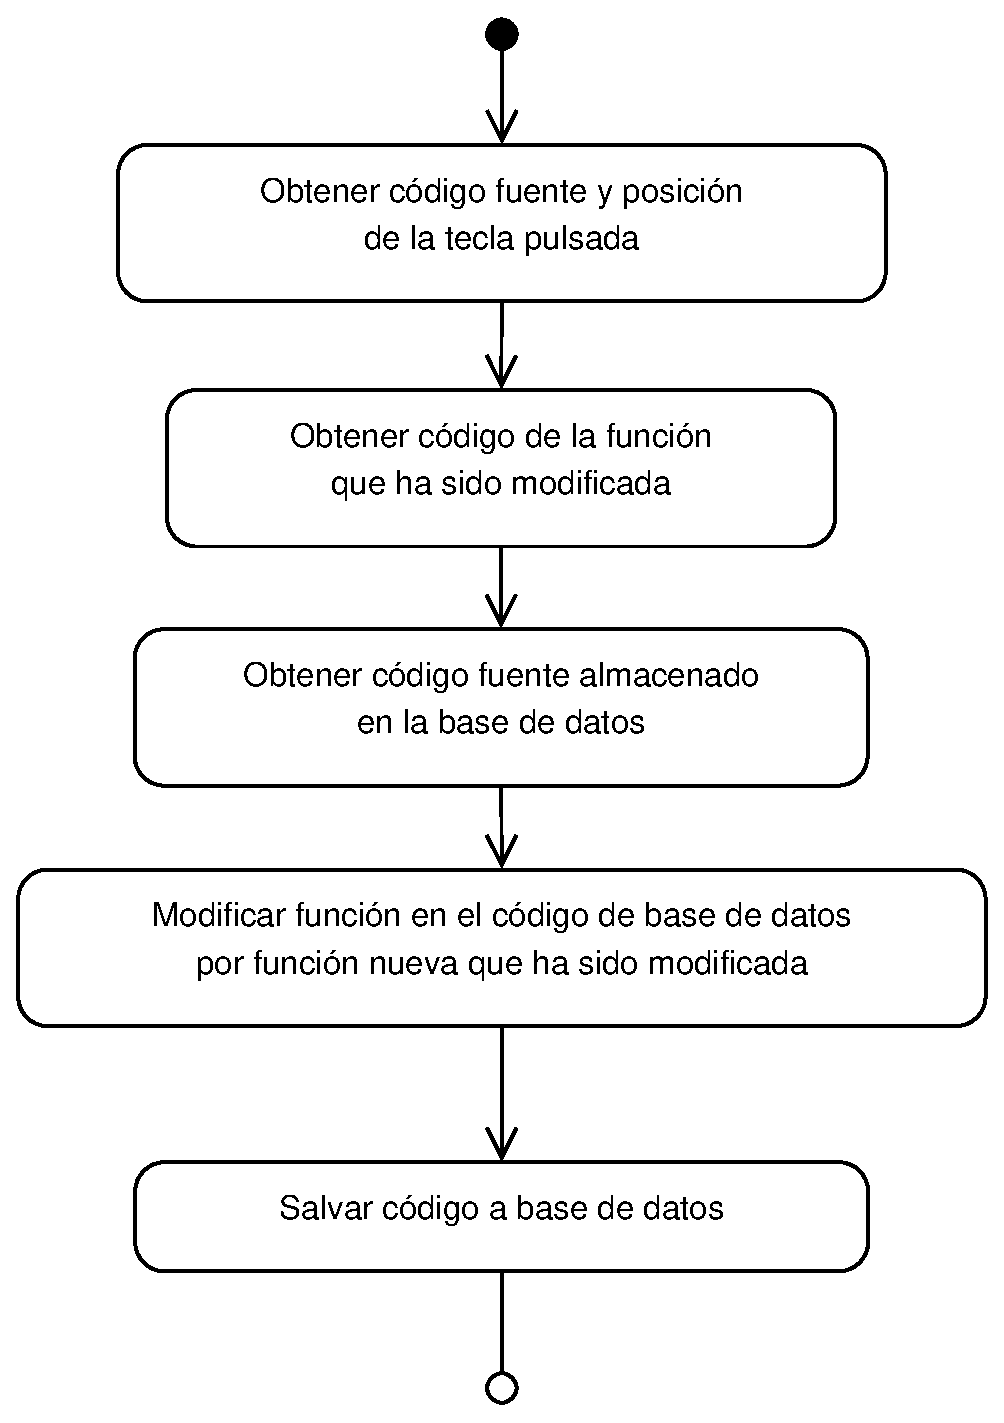
\includegraphics[width=0.5\textwidth]{./img/DiagramaA6.eps}
	\caption{Actividad sincronizar código}
\end{figure}

\newpage
\subsubsection{Actividad: Actualizar estadísticas}

Como se ha mostrado en la Figura 4.22, el usuario tendrá la posibilidad de consultar las estadísticas sobre su página de código. Estas estadísticas no son calculadas a la hora de realizar la consulta, sino que se van almacenando y actualizando en base de datos conforme se van produciendo, de este modo la carga de la operación de consulta es mucho menor y las operaciones únicamente son necesarias de realizar una vez. 

En el siguiente diagrama se muestra como se van calculando dichas estadísticas y almacenando en base de datos:

\begin{figure}[h]
	\centering
	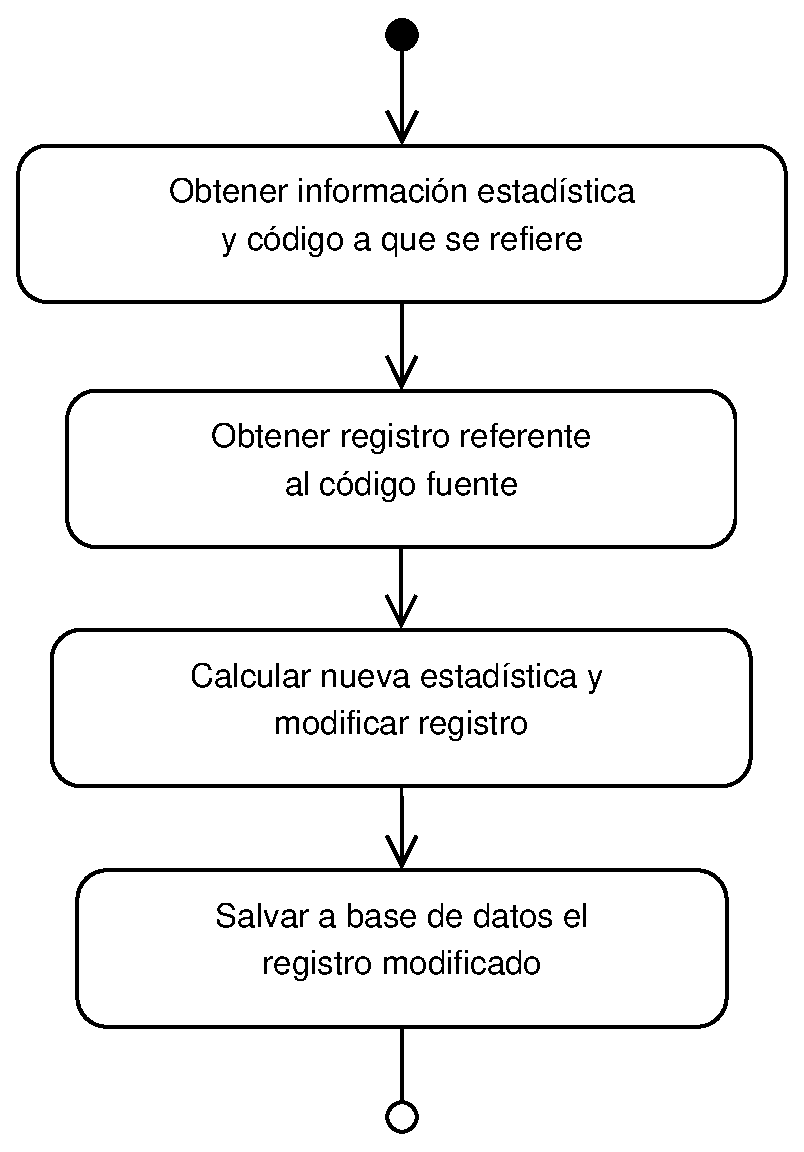
\includegraphics[width=0.4\textwidth]{./img/DiagramaA7.eps}
	\caption{Actividad actualizar estadísticas}
\end{figure}

\newpage

\section{Modelo de paquetes}

Para una mejor compresión de la arquitectura del sistema, los elementos del modelo de objetos se agrupan en paquetes. Un paquete organiza los objetos en grupos de modo que puedan ser manipulados de forma global. Cada paquete agrupa elementos cercanos semánticamente y funcionalmente. La visibilidad de los elementos del paquete va implícita en la propia especificación de cada elemento.

La interfaz del paquete la conforman todos aquellos elementos que son visibles fuera del paquete. Cada paquete posee un nombre único dentro del sistema. Un paquete puede contener subpaquetes cuyo nombre va precedido del nombre del paquete contenedor. Cada objeto pertenece exclusivamente a un único paquete. Un paquete forma un espacio de nombres, lo que significa que la nomenclatura de los elementos del mismo grupo no debe repetirse en el contexto de su paquete contenedor. Un paquete puede importar la interfaz de otro paquete para acceder a sus elementos. Esta importación es un permiso explícito de acceso en un solo sentido.

Un paquete puede ser representado gráficamente como una proyección de su modelo de contenido. Para la representación de cada paquete se hará uso de la notación gráfica de UML 2.0.

Para el caso de este proyecto tenemos una arquitectura cliente-servidor, por tanto se debe hacer una separación clara entre la interfaz de usuario del sistema que reside en el cliente y los datos persistentes del sistema que residen en el servidor.

\subsection{Paquete Cliente de Wikicode}

Este paquete representa el bloque cliente de la arquitectura. El bloque cliente visto desde el punto de vista físico estará formado por al menos un terminal que estará ejecutando la plataforma Moodle remotamente (navegador). Este terminal estará conectado con un servidor que será el módulo de Moodle que aceptará las peticiones del usuario.

\subsection{Paquete Servidor/Cliente Wikicode-Mod de Wikicode}

Esta parte representa al módulo de Moodle que actúa como servidor aceptando las peticiones del usuario y sirviendo de interfaz de entrada para la edición de código. Sin embargo, este servidor también actuará como cliente pues será el que realice las peticiones de sincronización de datos y salvado en base de datos. 

De esta manera, este módulo servidor/cliente deberá hacer lo siguiente:

\begin{itemize}
	\item Aceptar las peticiones del usuario.
	\item Obtener los registros de base de datos conforme a las peticiones de los usuarios.
	\item Hacer de interfaz de entrada a la hora de edición del código fuente.
	\item Enviar la petición de sincronización de código mediante un paquete JSon y el método Get\footnote{\textbf{Get: }Método de petición HTTP el cual pide una representación del recurso especificado.}.
	\item Enviar la petición de escritura en la conversación agrupada como chat mediante el método Post\footnote{\textbf{Post: }Método de petición HTTP el cual somete los datos a que sean procesados para el recurso identificado. Los datos se incluirán en el cuerpo de la petición.}.
	\item Llamar al compilador externo y leer la salida del fichero de intercambio.
\end{itemize}

La finalidad de este bloque es realizar una separación entre la aplicación que maneja la sincronización del código fuente y el sistema de gestión de cursos consiguiendo la independencia de ambos. Esta independencia es fundamental pues permite utilizar la aplicación de sincronización para cualquier otra plataforma que no sea Moodle.

\subsection{Paquete Servidor Wikicode-Synchronizer de Wikicode} 

El tercer bloque consiste en una clase que recoge el código y la posición del carácter modificado y la petición de sincronización o bloqueo. Una vez recogida la información, realiza los algoritmos necesarios para sincronizar el código fuente para que actúe de modo colaborativo. Una vez los datos se han sincronizado se almacenan en base de datos para que el bloque \emph{Wikicode-Mod} pueda tener acceso a ellos siempre que los necesite. También se enviará la información sincronizada como un paquete JSON para que dicho bloque no tenga que acceder de manera secuencial a base de datos.

\newpage
\subsection{Diagrama de paquetes}

El diagrama de paquetes correspondiente es el siguiente:

\begin{figure}[h]
	\centering
	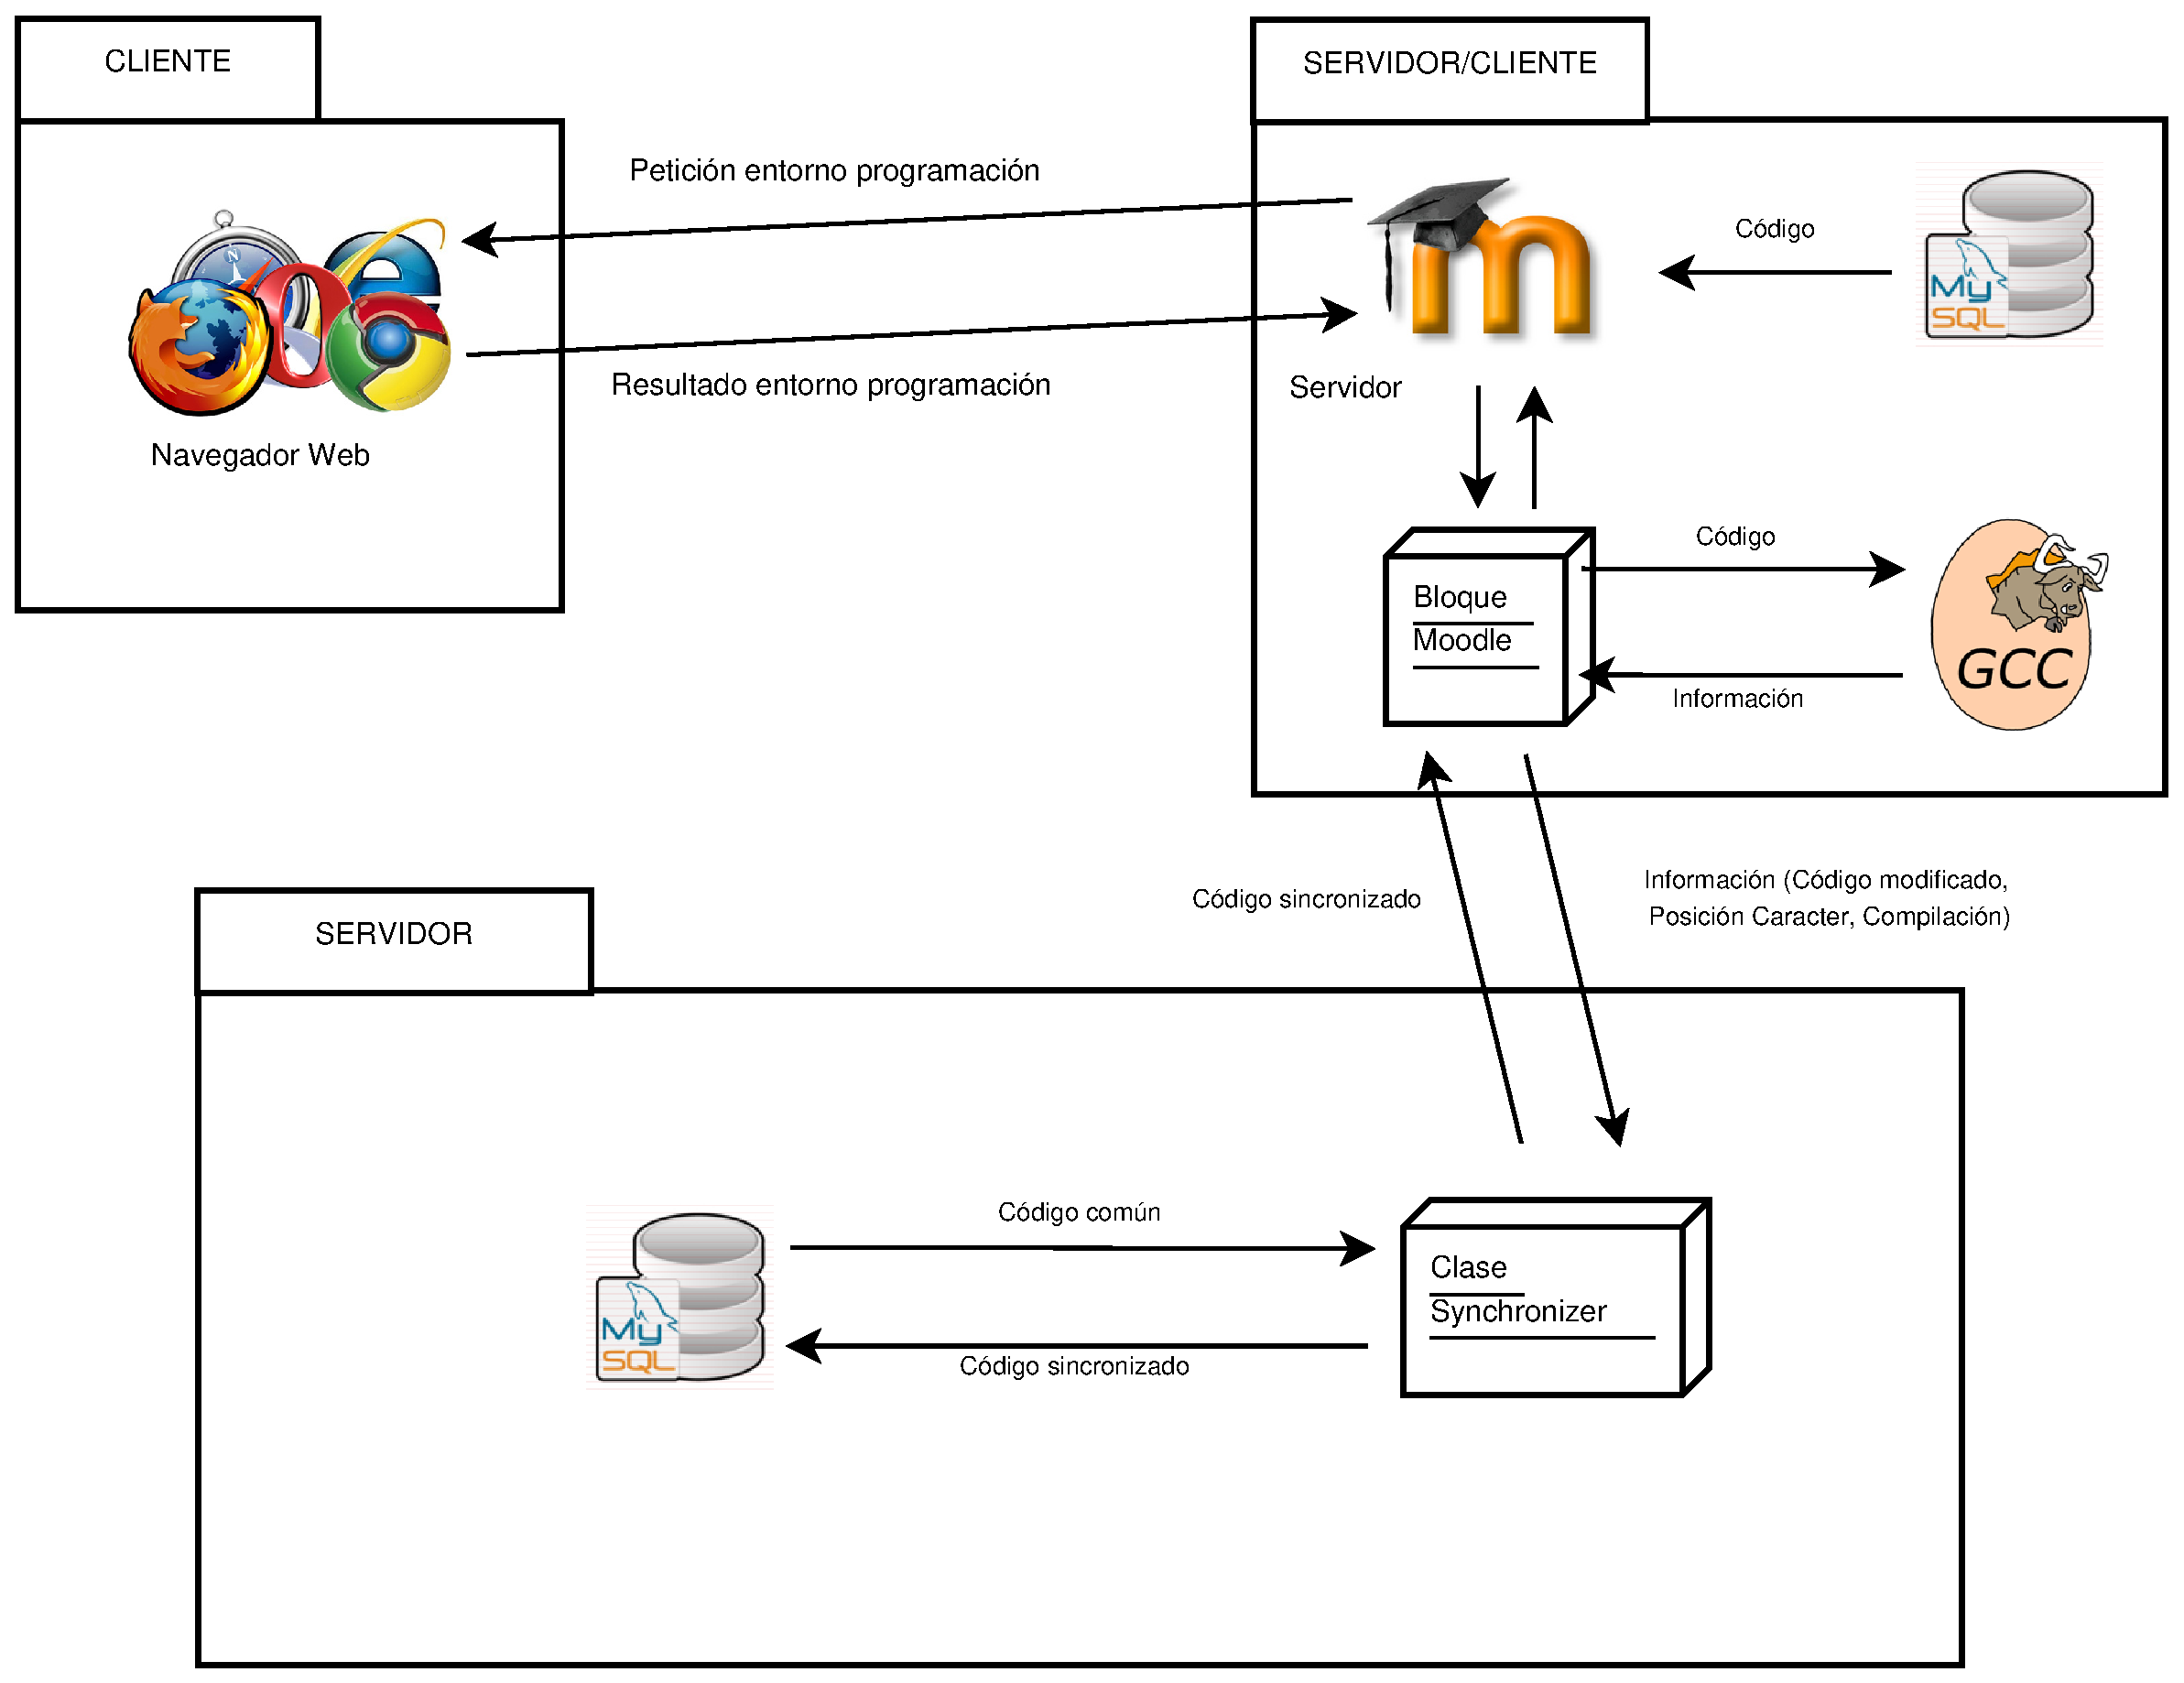
\includegraphics[width=\textwidth]{./img/diagramapaquetes.eps}
	\caption{Diagrama de paquetes}
\end{figure}


















































